\chapter{Grafische Darstellung von Daten -- Die MatPlotLib}
\label{chp:Matplotlib}
\epigraph{
	Real life seems to have no plots.
}{Ivy Compton-Burnett}

Menschen sind unheimlich gut darin, Bilder zu interpretieren. Computer haben ihre Stärke in der Auswertung von rohen Zahlen. Um nun die Früchte unserer Datenverarbeitung mit Python zu ernten, wollen wir Daten als graphische Plots ausgeben. Ein einfach zu bedienendes Mittel hierzu ist die MatPlotLib bzw. das Untermodul PyPlot. Das Modul MatPlotLib bietet tatsächlich so viele Funktionen, dass damit ein eigenständiger Kurs gefüllt werden könnte. Hier soll Ihnen eine Basis gezeigt werden, mit der Sie die häufigsten Aufgaben lösen können, und auf der Sie im Selbststudium leicht aufbauen können.

Eine erste Übersicht über die Funktionen der MatPlotLib finden Sie auch unter \url{https://matplotlib.org/tutorials/introductory/pyplot.html}.

\section{Grundlagen}
An dieser Stelle möchte ich Ihnen zuerst einen einfachen Code zeigen, und diesen dann Zeile für Zeile \enquote{entziffern}:

\begin{codebox}[Beispiel: Einfacher Plot, width=.55\linewidth, nobeforeafter, equal height group = grpXmpSimplePlot]
\begin{minted}[linenos]{python3}
import math
import matplotlib.pyplot as plt

N = 100
X = [(x - N/2) / 10 for x in range(N)]
Y = [math.sin(x) for x in X]

plt.plot(X, Y)
plt.show()
\end{minted}
\end{codebox}
%
\begin{tcolorbox}[title=Ausgabe: Einfacher Plot, width=.45\linewidth, nobeforeafter, equal height group = grpXmpSimplePlot]
	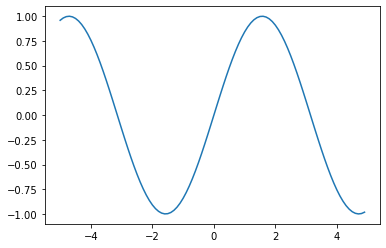
\includegraphics[width=\linewidth]{./gfx/plt-sin}
	\captionof{figure}{Einfacher Plot der MatPlotLib}
\end{tcolorbox}

In den Zeilen 1 und 2 laden wir Module -- zum einen das Modul \inPy{math}, mit dem wir die Daten generieren, die auf unserem Plot erscheinen sollen, und zum anderen die MatPlotLib. Tatsächlich handelt es sich dabei um ein extrem umfangreiches Paket, weswegen wir nur einen Teil davon in unser Projekt integrieren: Das Untermodul \inPy{pyplot}\footnote{Die MatPlotLib enthält Code zum Fenstermanagement, zur Interpolation von Kurven, Umgang mit Dateien, ... Alle diese Features bilden den Unterbau von \inPy{pyplot}, müssen aber nicht \enquote{offengelegt} werden, um für uns nützlich zu sein. Während \inPy{pyplot} intern alle diese Objekte und Funktionen benutzt und korrekt verwaltet, können wir uns auf das \emph{Interface} konzentrieren, das uns \inPy{pyplot} auf all diese Features bietet.}. Da dieser Modulname \inPy{matplotlib.pyplot} eher unhandlich ist, hat es sich eingebürgert, \inPy{plt} als Kurzname hierfür zu verwenden.

In den kommenden drei Zeilen generieren wir Werte, die schließlich geplottet werden sollen. \inPy{X} und \inPy{Y} sind jeweils Listen mit \inPy{N = 100} Elementen. Die Werte in \inPy{X} sind einfach gleichverteilte Werte im Abstand von \texttt{0.1}, rund um die \texttt{0} herum. Die Werte in \inPy{Y} enthalten jeweils den Sinus dieser \inPy{X}-Werte. Bis hierhin also haben wir noch nichts Neues gesehen.

In Zeile 8 wird nun die Funktion \inPy{plot} aus dem Modul \inPy{plt} aufgerufen. Diese Funktion bereitet alles vor, das nötig ist, um einen Plot zu generieren: Ein Arbeitsfenster, Achsen mit Beschriftung, Datenpunkte in den Graphen eintragen, ... All das wird aber nur im Arbeitsspeicher vorbereitet, jedoch noch nicht sichtbar gemacht. Grund hierfür ist, dass wir die Standard-Einstellungen noch abändern könnten: eine andere Linienfarbe, Skalierung, Bemaßung, \ldots Wenn jede Änderung in Echtzeit auf dem Bildschirm umgesetzt würde, hätte dies ein unangenehmes Flackern zur Folge, bevor der Plot endlich fertig aufgebaut ist. Stattdessen müssen wir manuell festlegen, wann unser Plot fertig beschrieben ist, \ie wann er auf dem Bildschirm erscheinen soll. Dies geschieht in Zeile 10.

Im einfachsten Fall müssen wir also folgende Arbeitsschritte erledigen:
\begin{itemize}
\item Das Modul \texttt{matplotlib.pyplot} laden
\item X- und Y-Werte als getrennte Listen vorbereiten
\item Die Funktion \texttt{plot} aufrufen
\item Die Funktion \texttt{show} aufrufen
\end{itemize}

Tatsächlich ist das Vorbereiten von X-Werten \emph{streng genommen} sogar überflüssig:

\begin{codebox}[Beispiel: Einfacher Plot ohne X-Werte, width=.55\linewidth, nobeforeafter, equal height group = grpXmpSimplePlotSansX]
\begin{minted}[linenos]{python3}
import matplotlib.pyplot as plt

N = 100
Y = [(x - 50) * x for x in range(N)]

plt.plot(Y)
plt.show()
\end{minted}
\end{codebox}
%
\begin{tcolorbox}[title=Ausgabe: Einfacher Plot ohne X-Werte, width=.45\linewidth, nobeforeafter, equal height group = grpXmpSimplePlotSansX]
	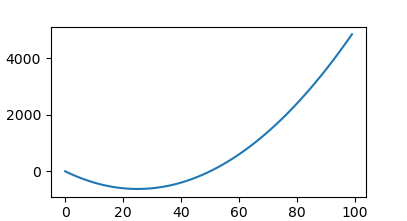
\includegraphics[width=\linewidth]{./gfx/plt-square}
	\captionof{figure}{Einfacher Plot ohne explizite x-Werte}
\end{tcolorbox}

Wenn keine X-Werte angegeben werden, erhalten wir zwar einen \enquote{sinnvollen} Plot; Python hat jedoch natürlich keine Möglichkeit, zu entscheiden, welcher Wert an welche Position gehört. Daher geht der Plotter hier davon aus, dass die Werte bei \inPy{x=0} beginnen und jeweils einen Abstand von \inPy{1} zueinander haben.

Folgen zwei \texttt{plot()}-Befehle direkt aufeinander ohne ein \texttt{show()} dazwischen, so werden beide Graphen auf denselben Plot gezeichnet. Jeder Plot bekommt dabei seine eigene Farbe. Eine Legende wird jedoch nicht \emph{automatisch} angezeigt.

\begin{codebox}[Beispiel: Zwei Graphen im selben Plot, width=.55\linewidth, nobeforeafter, equal height group = grpXmpSimplePlotTwoFunc]
\begin{minted}[linenos]{python3}
import matplotlib.pyplot as plt

N = 100
W = 10
X = [(x - N/2) / W for x in range(N)]
Y = [(x - W/2) * x for x in X]

plt.plot(X, Y)
plt.plot(X, [2 * y for y in Y])

plt.show()
\end{minted}
\end{codebox}
%
\begin{tcolorbox}[title=Ausgabe: Zwei Graphen im selben Plot, width=.45\linewidth, nobeforeafter, equal height group = grpXmpSimplePlotTwoFunc]
	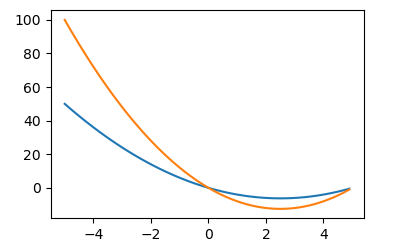
\includegraphics[width=\linewidth]{./gfx/plt-twoFuncs}
	\captionof{figure}{Zwei Graphen}
\end{tcolorbox}

\section{Einfache Formatierungen und andere Plot-Arten}
Die folgenden Abschnitte stellen eine Auswahl an Themen dar; für eine volle Übersicht der Features von MatPlotLib-Plots siehe \url{https://matplotlib.org/3.1.0/api/_as_gen/matplotlib.pyplot.plot.html}.

\subsection{Format-Angaben im Befehl \texttt{plot}}
Es wurde schon angesprochen, dass die Standard-Einstellungen der MatPlotLib nicht übernommen werden müssen. Im einfachsten Fall können wir direkt im \texttt{plot}-Befehl eine andere Linienfarbe und -form festlegen: Nach den Y-Werten kann ein optionaler String übergeben werden, in dem diese Information enthalten ist:
\mint{python3}{plt.plot(X, Y, "r--")}
weist die MatPlotLib dazu an, den Plot in Rot mit Strichlinien zu zeichnen. Dagegen steht
\mint{python3}{plt.plot(X, Y, "b-.")}
für einen Graphen aus blauen Punkten, die durch mit einer Linie verbunden sind. Folgende Zeichen werden verstanden und können auch miteinander kombiniert werden:

\begin{tcolorbox}[title=Format-Strings für \texttt{plt.plot()}]
\textbf{Punktarten}
\vspace{-6pt}
\begin{center}
	\begin{tabular}{cc|cc|cc}
		Symbol     & Punkt         & Symbol                    & Punkt            & Symbol     & Punkt            \tabcrlf
		\texttt{,} & Pixel         & \texttt{.}                & kleiner Punkt    & \texttt{o} & großer Punkt     \\
		\texttt{s} & Quadrat       & \texttt{d}                & schmale Raute    & \texttt{D} & breite Raute     \\
		\texttt{p} & Fünfeck       & \texttt{h}                & Sechseck stehend & \texttt{H} & Sechseck liegend \\
		\texttt{|} & Strich        & \texttt{+}                & Plus             & \texttt{x} & Kreuz            \\
		\texttt{<} & Dreieck links & \texttt{>}                & Dreieck rechts   & \texttt{*} & Stern            \\
		\texttt{v} & Dreieck unten & \texttt{\textasciicircum} & Dreieck oben                                     \\
	\end{tabular}
\end{center}

\textbf{Linienarten}
\vspace{-15pt}
\begin{center}
	\begin{tabular}{cc|cc|cc|cc}
		Symbol     & Linie        & Symbol      & Linie       & Symbol     & Linie     & Symbol      & Linie       \tabcrlf
		\texttt{-} & durchgezogen & \texttt{--} & gestrichelt & \texttt{:} & gepunktet & \texttt{-.} & strichpunkt \\
	\end{tabular}
\end{center}
\end{tcolorbox}
%
\begin{tcolorbox}
\textbf{Farben}
\begin{center}
	\begin{tabular}{cc|cc|cc|cc}
		Symbol     & Farbe   & Symbol     & Farbe   & Symbol     & Farbe & Symbol     & Farbe  \tabcrlf
		\texttt{b} & blau    & \texttt{c} & cyan    & \texttt{g} & grün  & \texttt{k} & schwarz \\
		\texttt{m} & magenta & \texttt{r} & rot     & \texttt{y} & gelb  & \texttt{w} & weiß    \\
	\end{tabular}
\end{center}

\captionof{table}{Formatstring-Elemente für \texttt{plot}}
\label{tab:PlotFormatStrings}
\end{tcolorbox}

Soll eine Kurve in einer Farbe gezeichnet werden, die nicht in Tabelle \ref{tab:PlotFormatStrings} aufgeführt sind, kann das Keyword-Argument \texttt{color} verwendet werden. Hier gibt man die Farbe als RGBA-String mit führendem Raute-Symbol an. Das bedeutet, dass der Rot- Grün- und Blau-Anteil der Farbe sowie die Deckkraft (\enquote{Alpha-Wert}) als zweistellige Hexadezimalzahl geschrieben wird und diese vier Zahlen dann aneinander gereiht werden. Für ein dunkles Rot kann man also schreiben:
\mint{python3}{plt.plot(X, Y, color="#7F0000FF")}
Dabei ist \texttt{7F} der Rot-Anteil (entspricht 50\% Intensität), \texttt{00} jeweils der Grün- und Blau-Anteil und \texttt{FF} die Deckkraft (entspricht 100\%).

\subsection{Legenden Anzeigen und Gitter anzeigen -- \texttt{legend}, \texttt{label} und \texttt{grid}}
Weiter ist es natürlich auch möglich, Graphen zu benennen und eine Legende anzeigen zu lassen. Dazu sind zwei Dinge nötig:
\begin{itemize}
\item Im Plot-Befehl muss mit dem Keyword-Argument \texttt{label} ein Titel angegeben werden
\item Mit dem Befehl \texttt{legend()} muss die Legende auch angezeigt werden:
\end{itemize}

\begin{codebox}[Beispiel: Plot mit Legende, width=.55\linewidth, nobeforeafter, equal height group = grpXmpSimplePlotLegend]
\begin{minted}[linenos]{python3}
import math
import matplotlib.pyplot as plt

N  = 100
X  = [(x - N/2) / 10 for x in range(N)]
Y1 = [math.sin(x) for x in X]
Y2 = [math.cos(x) for x in X]

plt.plot(X, Y1, label="Sinus")
plt.plot(X, Y2, label="Cosinus")

plt.legend()
plt.show()
\end{minted}
\end{codebox}
%
\begin{tcolorbox}[title=Ausgabe: Plot mit Legende, width=.45\linewidth, nobeforeafter, equal height group = grpXmpSimplePlotLegend]
	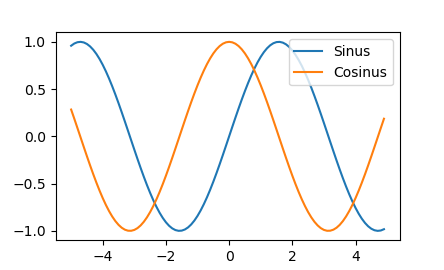
\includegraphics[width=\linewidth]{./gfx/plt-legend}
	\captionof{figure}{Plot mit Legende}
\end{tcolorbox}

Dem Befehl \texttt{plot} können noch viele weitere Keyword-Arguments mitgegeben werden, auf die hier nicht weiter eingegangen werden kann. Sie können sich bei Bedarf selbst die Bedeutung und Anwendung dieser Schlüsselworte anlesen; siehe hierzu die Dokumentation unter 
\url{https://matplotlib.org/2.1.2/api/_as_gen/matplotlib.pyplot.plot.html}

Um die Werte aus dem Plot besser ablesbar zu machen können auch Hilfslinien dazugeschalten werden. Dies erreicht der Befehl \texttt{grid}:

\begin{codebox}[Beispiel: Plot mit Gitterlinien, width=.55\linewidth, nobeforeafter, equal height group = grpXmpSimplePlotGrid]
\begin{minted}[linenos]{python3}
import math
import matplotlib.pyplot as plt

N  = 100
X  = [(x - N/2) / 10 for x in range(N)]
Y1 = [math.sin(x) for x in X]
Y2 = [math.cos(x) for x in X]

plt.plot(X, Y1, label="Sinus")
plt.plot(X, Y2, label="Cosinus")

plt.grid()

plt.legend()
plt.show()
\end{minted}
\end{codebox}
%
\begin{tcolorbox}[title=Ausgabe: Plot mit Gitterlinien, width=.45\linewidth, nobeforeafter, equal height group = grpXmpSimplePlotGrid]
	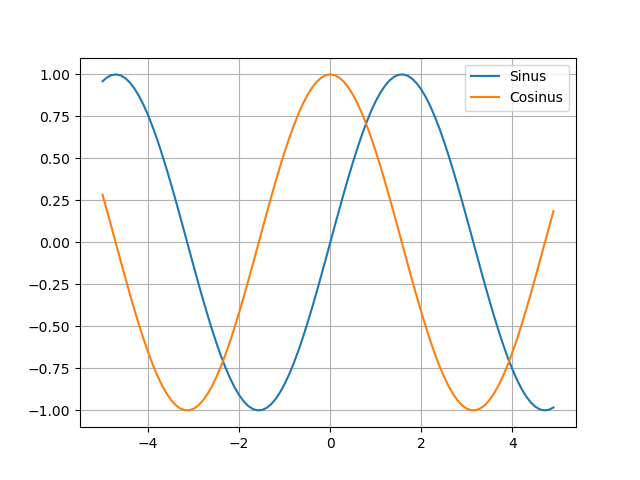
\includegraphics[width=\linewidth]{./gfx/plt-grid}
	\captionof{figure}{Plot mit Gitterlinien}
\end{tcolorbox}

\subsection{Titel und Achsenbeschriftung hinzufügen -- \texttt{title}, \texttt{xlabel}, \texttt{ylabel}}
Neben einer Legende sollten bei Plots auch Titel und Achsenbeschreibungen nicht fehlen. Diese lassen sich einfach über die Befehle \texttt{title}, \texttt{xlabel} und \texttt{ylabel} hinzugefügt werden. Das folgende Beispiel illustriert dies anhand der \emph{spektralen Strahlungsdichte eines idealen schwarzen Körpers}
\footnote{Crash-Kurs Physik:\\
Jeder Körper strahlt elektromagnetische Strahlung aus -- in einfachen Worten, jeder Körper leuchtet. Die Intensität und Lichtfarbe sind von der Temperatur abhängig. Heiße Körper glühen daher rot, sehr heiße Körper kommen sogar bis zur Weißglut; bei \enquote{kühlen} \SI{37}{\celsius} \enquote{leuchten} wir Menschen nur im Infrarot-Bereich. Aus diesem Grund sehen wir zwar nicht immer die Strahlung, die von jedem Körper ausgestrahlt wird, können diese aber trotzdem messen. Das gezeigte Programm berechnet die Intensität der einzelnen Licht-Wellenlängen, die ein Körper mit einer gegebenen Temperatur \texttt{T} ausstrahlt.\\
Streng genommen spielt hierbei auch die Farbe des Körpers eine Rolle; daher sprechen PhysikerInnen auch von \emph{Schwarzkörperstrahlung}. In der Praxis ist dieser Zusammenhang oft vernachlässigbar. Sekunden-Thermometer und Wärmebildkameras funktionieren nach diesem Prinzip: Ein Bild im Infraroten wird vom Objekt aufgenommen; die \enquote{Farbe} der gemessenen Strahlung wird dann als Temperatur interpretiert. Im gezeigten Plot liegt das Strahlungs-Maximum bei ca. \SI{20}{THz}, was einer Wellenlänge von \SI{15}{\micro\meter} entspricht -- weit außerhalb des Rahmens menschlicher Wahrnehmung, die zwischen ca. 400 und \SI{800}{\nano\meter} stattfindet, und damit in Übereinstimmung mit der täglichen Wahrnehmung, dass wir unsere Mitmenschen nicht glühen sehen.\\
Wenn Sie in Zeile 5 den Wert für \texttt{T} auf \inPy{5700} ändern und in Zeile 12 den Plot-Bereich auf \inPy{1e+15} erweitern, wird Ihnen das Spektrum der Sonne mit Maximum im sichtbaren Licht dargestellt.}:

\begin{codebox}[Beispiel: Plot mit Titel und Labels]
\begin{minted}[linenos]{python3}
import math
import matplotlib.pyplot as plt

h  = 6.62607015e-34     # Planck constant
T  = 300                # temperature in Kelvin
c  = 299792458          # speed of light
kB = 1.380649e-23       # Boltzmann constant

spectralDensity = lambda nu : ((2 * h * nu**3) / (c**2))  / \
                              (math.exp((h * nu) / (kB * T)) - 1)
\end{minted}
\end{codebox}
%
\begin{codebox}[]
\begin{minted}[linenos, firstnumber=last]{python3}
X = [x for x in range(1, int(1e+14), int(1e+10))]
Y = [spectralDensity(x) for x in X]

plt.title("Schwarzkörperstrahlung")
plt.xlabel("Strahlungsfrequenz in Hz")
plt.ylabel("Intensität in W/m²")

plt.plot(X, Y)
plt.show()
\end{minted}
\end{codebox}
%
\begin{tcolorbox}[title=Ausgabe: Plot mit Titel und Labels]
	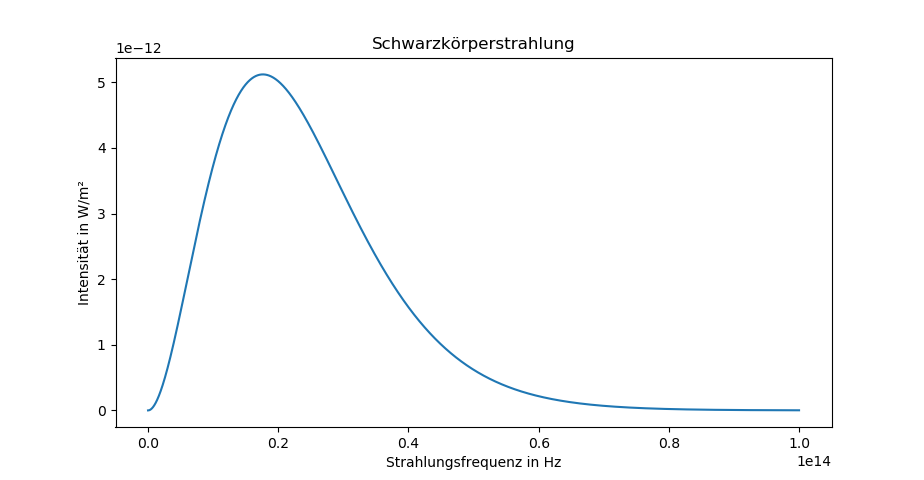
\includegraphics[width=\linewidth]{./gfx/plt-labels}
	\captionof{figure}{Plot mit Titel und Achsenbeschriftungen}
\end{tcolorbox}

Siehe \url{https://matplotlib.org/3.1.1/api/_as_gen/matplotlib.axes.Axes.legend.html#matplotlib.axes.Axes.legend} für weitere Optionen zum Befehl \texttt{legend}.

\subsection{Skalierung der Achsen -- \texttt{xscale}, \texttt{yscale} und \texttt{xlim}, \texttt{ylim}}
Wenn Plots einen großen Wertebereich abdecken, kann es sinnvoll sein, die Werte \emph{logarithmisch} aufzutragen. Eine oder mehrere Achsen werden dabei verzerrt, um über mehrere Größenordnungen hinweg Änderungen gut zu verfolgen. Hierzu dienen die Befehle \texttt{xscale} und \texttt{yscale}.

\begin{codebox}[Beispiel: Linearer und Logarithmischer Plot]
\begin{minted}[linenos]{python3}
import matplotlib.pyplot as plt

W  = 500
X  = [x / 10 for x in range(-W, W)]
Y1 = [2 ** x for x in X]
Y2 = [x ** 7 for x in X]
\end{minted}
\end{codebox}
%
\begin{codebox}[]
\begin{minted}[linenos, firstnumber=last]{python3}
plt.title("Linear Plot")
plt.plot(X, Y1, label="exponential")
plt.plot(X, Y2, label="power")
plt.legend()
plt.show()

plt.title("Logarithmic Plot")
plt.yscale("log")
plt.plot(X, Y1, label="exponential")
plt.plot(X, Y2, label="power")
plt.legend()
plt.show()
\end{minted}
\end{codebox}

\begin{tcbraster}[raster columns=2,
                  raster equal height,
                  nobeforeafter,
                  raster column skip=0.5cm]
\begin{tcolorbox}[title=Lineare Auftragung]
	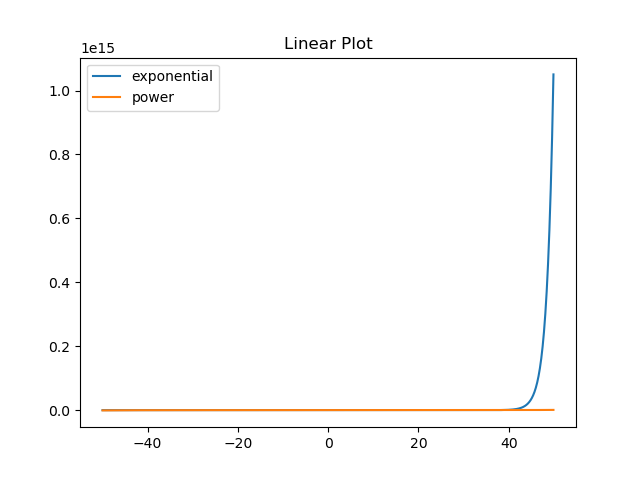
\includegraphics[width=\linewidth]{./gfx/plt-linear}
	\captionof{figure}{Linearer Plot}
	\label{gfx:PlotLinear}
\end{tcolorbox}
%
\begin{tcolorbox}[title=Logarithmische Auftragung]
	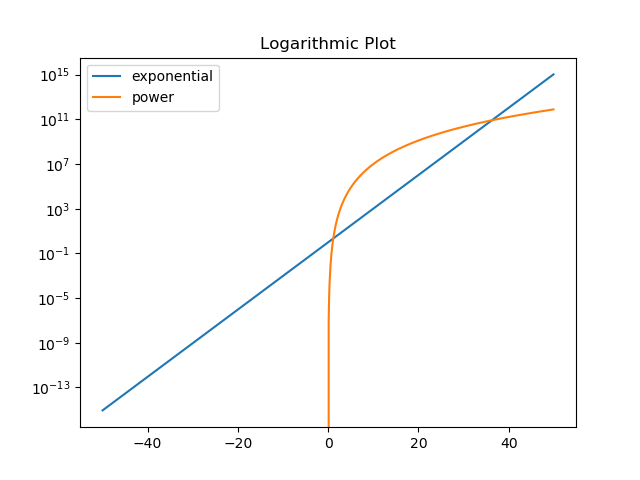
\includegraphics[width=\linewidth]{./gfx/plt-logarithmic}
	\captionof{figure}{Logarithmischer Plot}
	\label{gfx:PlotLogarithmic}
\end{tcolorbox}
\end{tcbraster}

In Abbildung \ref{gfx:PlotLinear} können wir kaum Details erkennen: Beide Plots bleiben \enquote{nahe} an der Null, bis die Exponentialfunktion irgendwann \enquote{explodiert}. Erst bei der logarithmischen Auftragung (Abbildung \ref{gfx:PlotLogarithmic}) sehen wir, dass das Polynom (orange Linie) zeitweise sogar größer ist als die Exponentialfunktion.

Wir haben diese Verzerrung erreicht, indem wir in Zeile 19 die y-Achse logarithmisch skaliert haben. Ebenso könnten wir mit \inPy{plt.xscale("log")} auch die x-Achse verzerren.

Der Logarithmus von 0 oder negativen Werten ist nicht definiert\footnote{liebe MathematikerInnen: natürlich beziehe ich mich auf den reellwertigen Logarithmus bzw. auf den Hauptzweig des Logarithmus.}. Um dennoch mit Werten umzugehen, die das Vorzeichen wechseln können und aber sinnvoller logarithmisch aufgetragen werden sollten, existiert auch die Option \inPy{"symlog"}. Hier wird jeweils der Logarithmus \emph{des Betrags} der Werte aufgetragen; abhängig vom Vorzeichen geschieht dies dann nach oben oder unten (\inPy{plt.yscale("simlog")} bzw. nach links oder rechts (\inPy{plt.xscale("simlog")}. Werte nahe der 0 werden linear aufgetragen. Was als nahe der 0 gelten soll, kann mit den Keyword-Arguments \texttt{linthreshx} bzw. \texttt{linthreshy} bestimmt werden. Die Grenzen des linearen bereichs sind auch als Hilfslinien sichtbar, wenn \texttt{grid} benutzt wird.

Für statistische Auswertungen ist manchmal auch der \enquote{Logit} einer Wahrscheinlichkeit interessant ($\text{logit}(y) = \log(\frac{y}{1-y})$). Für y-Werte zwischen 0 und 1 kann so auch \inPy{plt.xscale("logit")} eingestellt werden.

\begin{codebox}[Beispiel: Auftragung mit \texttt{symlog}]
\begin{minted}[linenos]{python3}
import math
import matplotlib.pyplot as plt

W  = 500
X  = [x / 10 for x in range(-W, W)]
Y1 = [math.sin(x) for x in X]
Y2 = [x / 10      for x in X]

plt.xscale("symlog")
plt.plot(X, Y1)
plt.plot(X, Y2)
plt.grid()
plt.show()

plt.xscale("symlog", linthreshx=10)
plt.plot(X, Y1)
plt.plot(X, Y2)
plt.grid()
plt.show()
\end{minted}
\end{codebox}

\begin{tcolorbox}[title=Auftragung mit \texttt{symlog}]
	\begin{minipage}{.49\linewidth}
		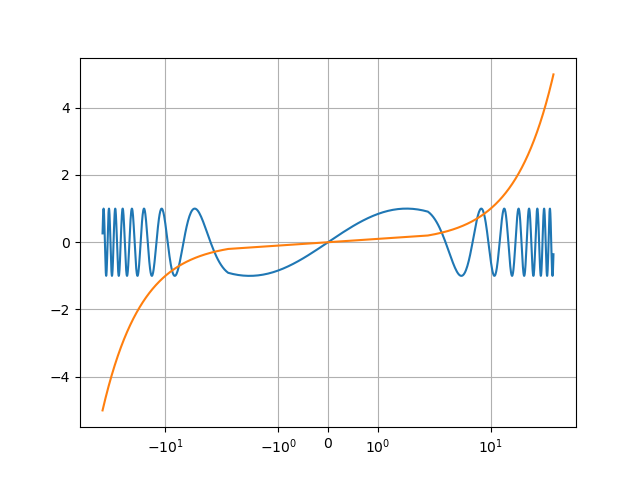
\includegraphics[width=\linewidth]{./gfx/plt-symlog}
		\captionof{figure}{symmetrisch-logarithmische Auftragung mit Standard-Schranke für lineare Auftragung}
		\label{gfx:PlotSymlog}
	\end{minipage}
%
	\begin{minipage}{.49\linewidth}
		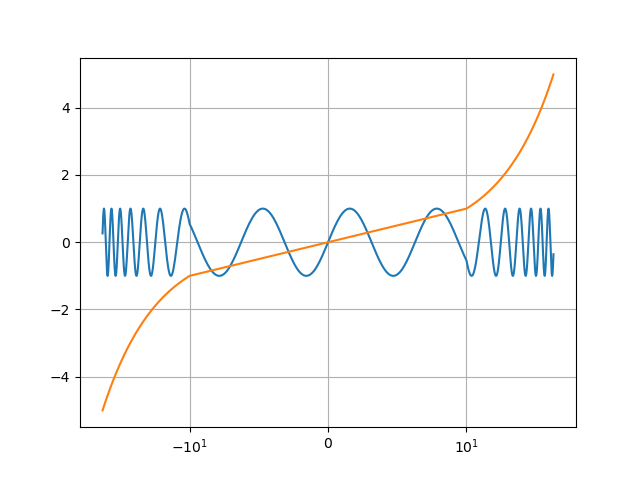
\includegraphics[width=\linewidth]{./gfx/plt-symlog-threshold}
		\captionof{figure}{symmetrisch-logarithmische Auftragung mit höherer Schranke für lineare Auftragung}
		\label{gfx:PlotSymlog-Threshold}
	\end{minipage}
\end{tcolorbox}

In Ähnlicher Manier kann mit \texttt{xlim} und \texttt{ylim} festgelegt werden, in welchen Grenzen die X- und Y-Achse skaliert werden sollen, unabhängig von den \enquote{Ausmaßen} des tatsächlichen Graphen. Der Graph füllt dann nicht mehr die gesamte Plot-Fläche aus, bzw. wird gegebenenfalls abgeschnitten:

\begin{codebox}[Beispiel: Manuell gewählte Plot-Skalierung, width=.55\linewidth, nobeforeafter, equal height group = grpXmpSimplePlotScale]
\begin{minted}[linenos]{python3}
import math
import matplotlib.pyplot as plt

N = 100
X = [(x - N/2) / 10 for x in range(N)]
Y = [math.sin(x) for x in X]

plt.plot(X, Y)
plt.xlim(-6  , +6)
plt.ylim(-0.7, +3)
plt.grid()
plt.show()
\end{minted}
\end{codebox}
%
\begin{tcolorbox}[title=Manuell gewählte Plot-Skalierung, width=.45\linewidth, nobeforeafter, equal height group = grpXmpSimplePlotScale]
	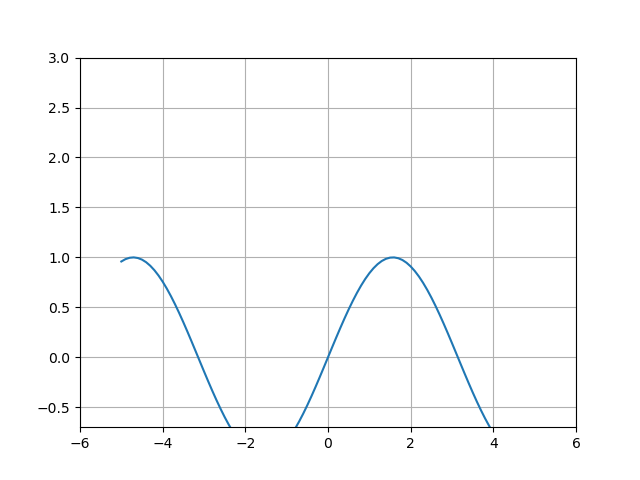
\includegraphics[width=\linewidth]{./gfx/plt-limits}
	\captionof{figure}{Manuelle Skalierung}
\end{tcolorbox}

\subsection{Andere Plot-Arten}
Neben Kurven in einem X-Y-Diagramm kann die MatPlotLib auch andere Arten von Visualisierungen erzeugen.

\subsubsection{Balkendiagramme}
Barplots oder Balkendiagramme verhalten sich ähnlich wie die Punkt- oder Liniendiagramme, die im letzten Abschnitt gezeigt wurden. Alle oben erwähnten Befehle funktionieren auch hier, außerdem kann auch das Keyword-Argument \texttt{color} verwendet werden. Erstellt werden Barplots mit den Befehlen \texttt{bar} (vertikale Balken) und \texttt{barh} (horizontale Balken). Die \enquote{X-Werte} dürfen für Barplots auch Strings enthalten, und werden entsprechend als Beschriftung angebracht. Wie schon bei den Liniendiagrammen können auch hier mehrere Graphen auf demselben Plot dargestellt werden.

\begin{codebox}[Beispiel: Barplots]
\begin{minted}[linenos]{python3}
import matplotlib.pyplot as plt

X = ["Smoot", "Fnord", "R'lyeh"]
Y = [random.randint(0, 11) for x in X]   # this one goes up to eleven

plt.bar(X, Y, color="#0040B0FF")
plt.ylim(0, 11)
plt.show()

plt.barh(X, Y, color="#0040B0FF")
plt.xlim(0, 11)
plt.show()
\end{minted}
\end{codebox}
%
\begin{tcbraster}[raster columns=2,
                  raster equal height,
                  nobeforeafter,
                  raster column skip=0.5cm]
\begin{tcolorbox}[title=Vertikaler Barplot]
	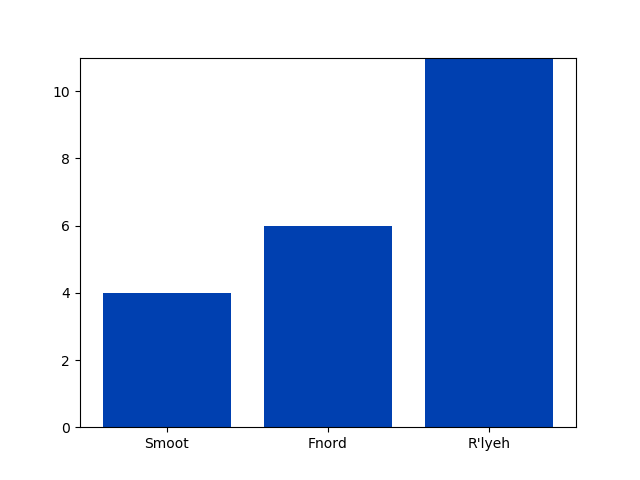
\includegraphics[width=\linewidth]{./gfx/plt-bars}
	\captionof{figure}{Vertikaler Barplot}
\end{tcolorbox}
%
\begin{tcolorbox}[title=Horizontaler Barplot]
	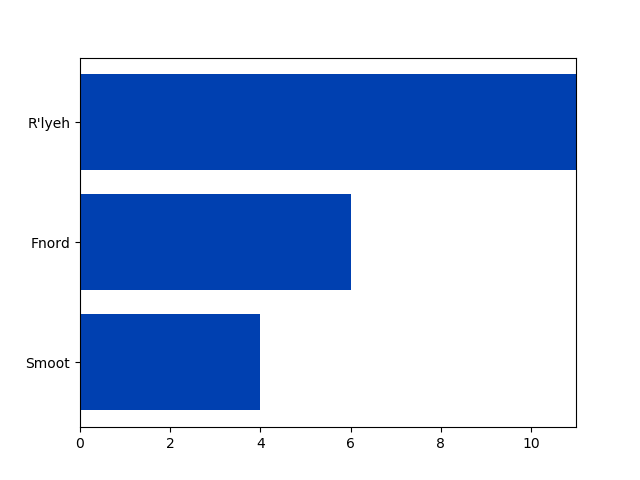
\includegraphics[width=\linewidth]{./gfx/plt-barh}
	\captionof{figure}{Horizontaler Barplot}
\end{tcolorbox}
\end{tcbraster}

Siehe auch \url{https://matplotlib.org/3.1.1/api/_as_gen/matplotlib.pyplot.bar.html} für weitere Details und \url{https://matplotlib.org/3.1.1/gallery/lines_bars_and_markers/bar_stacked.html} für ein weiteres Beispiel.

\subsubsection{Kuchendiagramme}
Kuchendiagramme sind die klassische Darstellungsform, wenn die Anteile verschiedener Beiträge zu einem Gesamten visualisiert werden sollen. Die MatPlotLib erlaubt das Erstellen solcher Diagramme mit dem Befehl \texttt{pie}. Wie auch schon zuvor kann im einfachsten Fall eine einfache \inPy{list} übergeben werden, um ein minimales Kuchendiagramm zu erstellen. Die Werte müssen sich dabei \emph{nicht} zu 100\% bzw. zu 1 aufaddieren.

\begin{codebox}[Beispiel: Einfaches Kuchendiagramm, width=.55\linewidth, nobeforeafter, equal height group = grpXmpSimplePie]
\begin{minted}[linenos]{python3}
import matplotlib.pyplot as plt

contributions = {
    "trial & error"               : 90,
    "searching the web"           : 50,
    "despair, fits of anger, etc" : 10,
    "writing small bits of code"  : 30,
    "brilliant ideas"             : 1
}

plt.pie( contributions.values() )
plt.show()
\end{minted}
\end{codebox}
%
\begin{tcolorbox}[title=Ausgabe: Einfaches Kuchendiagramm, width=.45\linewidth, nobeforeafter, equal height group = grpXmpSimplePie]
	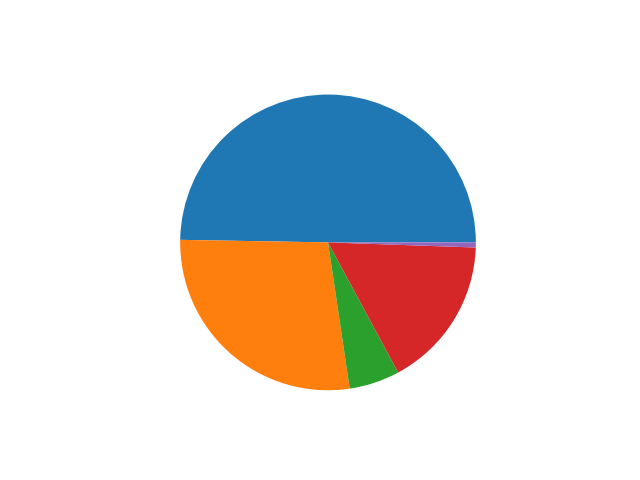
\includegraphics[width=\linewidth]{./gfx/plt-pie-simple}
	\captionof{figure}{Einfaches Kuchendiagramm der matplotlib}
\end{tcolorbox}

Selbstverständlich kann auch hier ein Titel mit \texttt{title} hinzugefügt werden. Die Befehle \texttt{xlabel} und \texttt{ylabel} erstellen tatsächlich Textfelder an den zu erwartenden Stellen, und können für Beschriftungen \enquote{missbraucht} werden. Labels funktionieren wie schon bei \texttt{plot} gezeigt, \ie über das optionale Argument \texttt{labels} werden Texte zugewiesen; der Befehl \texttt{legend} sorgt dafür, dass diese dann in einer Box angezeigt werden. Zusätzlich werden Labels direkt neben den Kuchenstücken angezeigt, wenn solche mit dem Keyword Argument \texttt{labels} als \inPy{list} übergeben werden. Dagegen hat der Befehl \texttt{grid} keine Effekt. 

Eine Auswahl an optionalen Argumenten für den Befehl \texttt{pie} ist in Tabelle \ref{tab:OptArgsPie} aufgeführt. Weitere Argumente sind unter \url{https://matplotlib.org/3.1.0/api/_as_gen/matplotlib.pyplot.pie.html} aufgeführt.

\begin{tcolorbox}[title=Auswahl an Optionalen Argumenten bei \texttt{pie}]
	\begin{tabularx}
		{\linewidth}
		{>{\ttfamily}p{.2\linewidth} | p{.2\linewidth} p{.5\linewidth}}
		\textrm{\textbf{Schlüsselwort}} & \textbf{Datentyp} & \textbf{Effekt} \tabcrlf
		labels & 
			\texttt{list} oder \texttt{tuple} &
			Liste von Strings, die neben jedem Kuchenstück angezeigt werden soll. Die Länge der Liste muss mit der Anzahl der Kuchenstücke
			 übereinstimmen.\\
		colors &
			\texttt{list} oder \texttt{tuple} &
			Liste von Strings mit Farbangaben. Farbangaben können entweder einzelne Buchstaben wie in Tabelle \ref{tab:PlotFormatStrings} sein, ausgewählte englische
			Farbnamen oder hexadezimale Farbangaben \\
		explode &
			\texttt{list} oder \texttt{tuple} &
			Liste von Zahlen, die angeben, wie weit jedes Kuchenstück vom Mittelpunkt abgesetzt sein soll in Einheiten des Kreisradius (\ie 0 bedeutet: Kuchenstück-Spitze
			berührt den Mittelpunkt; 1 bedeutet: Kuchenstück-Spitze würde den Rand des Kreises berühren) \\
		autopct &
			String oder Funktion &
			Wenn hier ein String übergeben wird, interpretiert die MatPlotLib diesen als Format-String (siehe Abschnitt \ref{sec:FormatStringsTable}).
			Bei einer Funktion dagegen wird erwartet, dass die Funktion eine Zahl zwischen 0 und 100 als Argument akzeptiert, und einen String zurückgibt, der eine
			Textentsprechung dieser Zahl enthält.
	\end{tabularx}
	\captionof{table}{Optionale Argumenten bei \texttt{matplotlib.pyplot.pie} (Auswahl)}
	\label{tab:OptArgsPie}
\end{tcolorbox}

\begin{codebox}[Beispiel: Verändertes Kuchendiagramm]
\begin{minted}[linenos]{python3}
import matplotlib.pyplot as plt

contributions = {
    "trial & error"                 : 99,
    "searching the web"             : 50,
    "despair, fits of anger, etc"   : 10,
    "writing small bits\n of code"  : 30,
    "brilliant ideas"               : 1
}

def percentToWords(x) :
    if        x <  5 : return "virtually nothing"
    elif  5 < x < 20 : return "a little"
    elif 20 < x < 50 : return "quite a bit"
    else             : return "the majority"

plt.title("Time Allocation in a coding project")
plt.xlabel("taken from experience")

plt.pie(
    contributions.values(),
    labels=contributions.keys(),
    colors=["#0000AAFF", "blue", "r", "green", "gold"],
    explode=(0, 0.1, 0, 0, .3),
    autopct=percentToWords
)
plt.show()
\end{minted}
\end{codebox}
%
\begin{tcolorbox}[title=Ausgabe: Verändertes Kuchendiagramm]
\begin{center}
	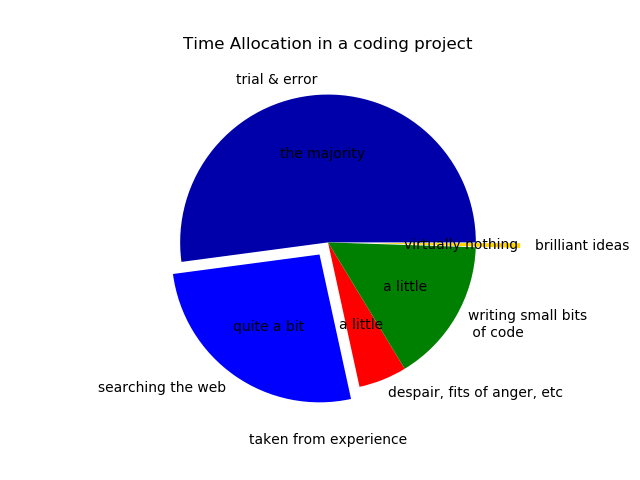
\includegraphics[width=.68\linewidth]{./gfx/plt-pie-args}
	\captionof{figure}{Kuchendiagramm mit Optionen}
\end{center}
\end{tcolorbox}

\subsubsection{Stackplots}
Wo eine Zusammensetzung über eine Zeit verfolgt werden soll, bietet sich die Darstellungsfomr \emph{stacked plot} an, die mit dem Befehl \texttt{stackplot} erstellt wird. Wie schon bei normalen Plots ist das erste, optionale Argument eine Liste von X-Werten. Danach können entweder mehrere eindimensionale Listen stehen, die als Y-Werte aufgetragen werden, oder eine zweidimensionale Liste:

\begin{codebox}[Beispiel: Stackplot]
\begin{minted}[linenos]{python3}
import csv
import matplotlib.pyplot as plt

years    = []
africa   = []
americas = []
asia     = []
europe   = []
oceania  = []
colors   = ["gold", "black", "red", "blue", "green"]

with open("annual-number-of-births-by-world-region.csv", "r") as handle :
    # Daten von https://ourworldindata.org/world-population-growth
    # Datei enthält Daten in der Form:
    # Year,Asia,Africa,America,Europe,Oceania
    # 1950,11071.722,8896.969,62638.002,11837.577,360.997
    # 1951,11178.006,9031.823,62344.074,11917.33,366.362
    # ...
      
    reader = csv.reader(handle)
    
    labels = next(reader)[1:]    # erste Zeile lesen;
                                 # Spaltenüberschriften ohne "Years" übernehmen

    for line in reader :         # verbleibende Zeilen einlesen
        years   .append(float(line[0])       )
        africa  .append(float(line[1]) / 1000)  # line[i] / 1000: Daten sind in
        americas.append(float(line[2]) / 1000)  # Tausend Geburten angegeben.
        asia    .append(float(line[3]) / 1000)  # Plot soll in Millionen sein.
        europe  .append(float(line[4]) / 1000)
        oceania .append(float(line[5]) / 1000)


plt.title ("annual number of births by world region")
plt.xlabel("year")
plt.ylabel("annual number of births in millions")
plt.legend(loc="upper left")
\end{minted}
\end{codebox}
%
\begin{codebox}[]
\begin{minted}[linenos, firstnumber=last]{python3}
plt.stackplot(
    years,
    asia, africa, americas, europe, oceania,
    labels=labels,
    colors=colors
)

# Alternative, erzeugt selbes Ergebnis:
# data = [asia, africa, americas, europe, oceania]
# plt.stackplot(years, data, labels = labels, colors=colors)

plt.show()
\end{minted}
\end{codebox}
%
\begin{tcolorbox}[title=Ausgabe: Stackplot]
\begin{center}
	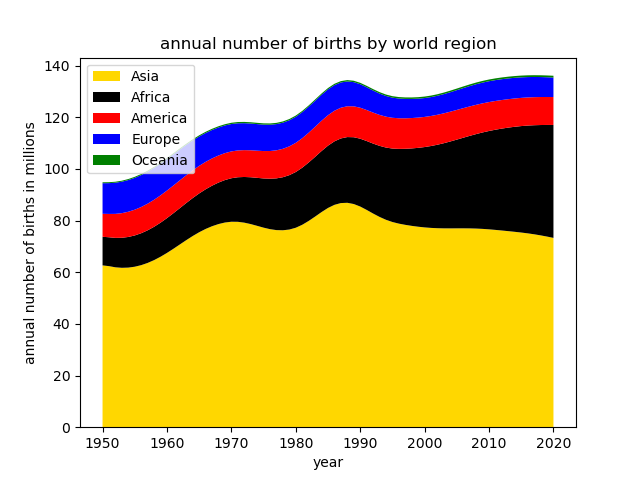
\includegraphics[width=.8\linewidth]{./gfx/plt-stackplot}
	\captionof{figure}{Stackplot: Anzahl Geburten über die Zeit je Kontinent}
\end{center}
\end{tcolorbox}

Für weitere Details, siehe \url{https://matplotlib.org/3.1.1/api/_as_gen/matplotlib.pyplot.stackplot.html}


\subsubsection{Scatterplots}
Scatterplots erlauben es, Orten in einer Fläche ein Gewicht zuzuweisen. Dem Befehl \texttt{scatter} können bis zu vier Parameter übergeben werden. Die ersten beiden davon sind X- und Y-Koordinaten der Punkte, die geplottet werden sollen, übergeben als \inPy{list}. Der dritte Parameter enthält eine \inPy{list} mit der Größe der Punkte und ist optional. Als vierten Parameter kann die Farbe der einzelnen Punkte als \inPy{list} übergeben werden.

\begin{codebox}[Beispiel: Scatterplot]
\begin{minted}[linenos]{python3}
import csv
import matplotlib.pyplot as plt

lat = []      # geographische Länge
lng = []      # geographische Breite
pop = []      # Einwohnerzahl
col = []      # Farbe

colors = {
    "primary" : "red",     # Bundeshauptstadt
    "admin"   : "blue",    # Landeshauptstadt
    "minor"   : "black"    # andere Stadt
}

# Größe des Punktes aus Einwohnerzahl berechnen: kleine Städte sollen dabei
# nicht "verschwinden"
sizer = lambda x : 0.5 if x < 10000 else x / 10000

with open("cities-locations-populations-Germany.csv", "r") as handle :
    # Daten von https://simplemaps.com/data/de-cities
    # Datei enthält Daten in der Form:
    # city,lat,lng,country,iso2,admin_name,capital,population,population_proper
    # Berlin,52.5167,13.3833,Germany,DE,Berlin,primary,3644826,3644826
    # Hamburg,53.5500,10.0000,Germany,DE,Hamburg,admin,1841179,1841179
    # ...
    
    reader = csv.reader(handle)
    
    next(reader)
    
    for line in reader :
            lat.append(float(line[1]))
            lng.append(float(line[2]))
            pop.append( sizer(float(line[7]))  )
            col.append( colors[line[6]] )

plt.figure(figsize=(6,7.5))
plt.title("Deutschland: Städte")
plt.xlabel("Geographische Länge")
plt.ylabel("Geographische Breite")
plt.scatter(lng, lat, pop, col)
plt.show()
\end{minted}
\end{codebox}
%
\begin{tcolorbox}[title=Ausgabe: Scatterplot]
\begin{center}
	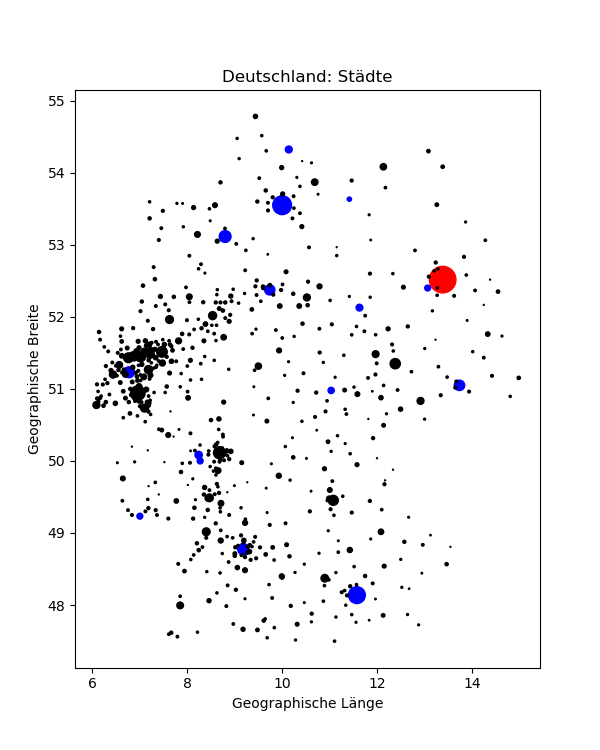
\includegraphics[width=.7\linewidth]{./gfx/plt-de}
	\captionof{figure}{Scatterplot: Städte Deutschlands}
\end{center}
\end{tcolorbox}

Siehe auch \url{https://matplotlib.org/3.1.0/api/_as_gen/matplotlib.axes.Axes.scatter.html}

\subsubsection{Histogramme}
Häufig wird dieselbe Simulation mehrfach mit verschiedenen Ausgangswerten durchgeführt. Wir erhalten so eine Liste von Ergebnissen. Oft interessiert uns dann, wie häufig ein bestimmtes Ergebnis erhalten wurde. 

Beispiel:\\
In der folgenden Liste:
\mint{python3}{[1, 5, 2, 1, 6, 2, 6, 8, 4]}
finden wir die folgende Häufigkeit der Zahlen:
\mint{python3}{{1:2, 2:2, 4:1, 5:1, 6:2, 8:1}}
Eine solche Aufschlüsselung nennt sich \emph{Histogramm}. In der Regel führen wir dann \emph{bins} ein, \ie Wertebereiche, die als eine Klasse gezählt werden sollen. Wollen wir also jeweils zwei aufeinanderfolgende Zahlen als eine Klasse zählen, so erhalten wir folgende Aufschlüsselung:
\mint{python3}{{1:4, 3:1, 5:3, 7:1}}

Mit der MatPlotLib können solche Histogramme automatisch erstellt\footnote{Tatsächlich erfolgt die Datenanalyse im Hintergrund mit dem Modul NumPy, das in Kapitel \ref{chp:Numpy} besprochen wird. Aus didaktischen Gründen wollen wir hier zuerst die MatPlotLib besprechen.} und als Plot dargestellt werden. Hierzu dient der Befehl \texttt{hist}. Als Parameter wird eine Liste von Ergebnissen übergeben, aus der automatisch das Histogramm berechnet und daraus ein Balkendiagramm erstellt. Rückgabewert von \texttt{hist} ist ein Tupel bestehend aus den \inPy{list}s\footnote{Eigentlich NumPy-Arrays; diese verhalten sich aber im Wesentlichen wie \inPy{list}s. Siehe Kapitel \ref{chp:Numpy} für Details.} \texttt{count} und \texttt{bins} sowie einem \texttt{Patch}-Objekt. In \texttt{count[i]} ist gespeichert, wie viele Ergebnisse jeweils in die \texttt{i}-te Klasse fallen; \texttt{bins[i]} gibt an, bei welchem Wert die \texttt{i}-te Klasse beginnt. Auf das \texttt{Patch}-Objekt kann hier nicht näher eingegangen werden.

\begin{codebox}[Beispiel: Einfaches Histogramm]
\begin{minted}[linenos]{python3}
import matplotlib.pyplot as plt

data = [1, 5, 2, 1, 6, 2, 6, 8, 4]

count, bins, patches = plt.hist(data)
print(bins)
print(count)
plt.show()
\end{minted}
\end{codebox}

\begin{tcbraster}[raster columns=2,
                  raster equal height,
                  nobeforeafter,
                  raster column skip=0.5cm]
\begin{cmdbox}[Konsolenausgabe: Einfaches Histogramm]
\begin{minted}{text}
[1.  1.7 2.4 3.1 3.8 4.5 5.2 5.9 6.6
  7.3 8. ]
[2. 2. 0. 0. 1. 1. 0. 2. 0. 1.]
\end{minted}
\end{cmdbox}
%
\begin{tcolorbox}[title=Plot: Einfaches Histogramm]
	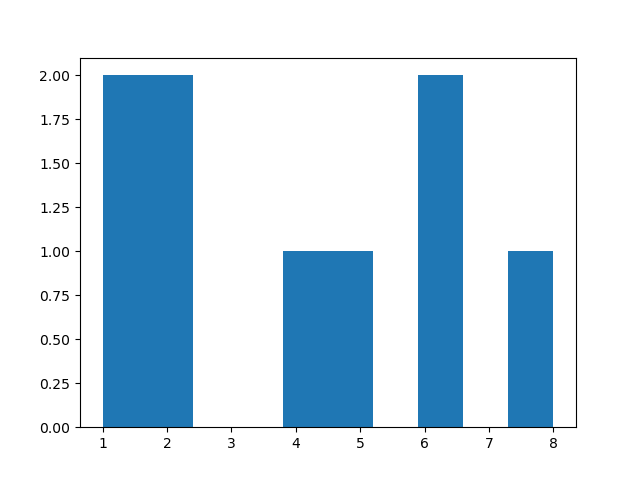
\includegraphics[width=\linewidth]{./gfx/plt-hist-simple}
	\captionof{figure}{Einfaches Histogramm}
\end{tcolorbox}
\end{tcbraster}

Der optionale \inPy{int}-Parameter \texttt{bins} gibt an, in wie viele Klassen diese Liste unterteilt werden soll. Über das Keyword-Argument \texttt{range} kann ein \inPy{tuple} übergeben werden, der die untere und obere Schranke für die Klassierung enthält. 

Hier sei ein beschränkter \emph{Random Walk} gezeigt: Ein Betrunkener geht \texttt{N} Schritte eine Straße entlang. Bei jedem Schritt wird er entweder nach links oder nach rechts torkeln; die Wahrscheinlichkeit für einen Schritt nach Links beträgt dabei \texttt{pleft}. Die Straße ist insgesamt \texttt{B} Schritte breit. Der Plot zeigt, wie wahrscheinlich der Betrunkene am Ende seines Laufs an einem 

\begin{codebox}[Beispiel: Drunk Walk als Histogramm]
\begin{minted}[linenos]{python3}
import random
import matplotlib.pyplot as plt

runs   = 10000
N      = 100
B      = 20
pLeft  = 0.5
drifts = [0] * runs

for run in range(runs) :
    drift  = 0
    for step in range(N) :
        r = random.uniform(0, 1)
    
        if r < pLeft :                      # Schritt nach links
            if drift != -B : drift -= 1
        else :                              # Schritt nach rechts
            if drift != +B : drift += 1
  
    drifts[run] = drift

data, bins, patches = plt.hist(drifts, 
                               bins=B+1, range=(-B-1, B+1),
                               histtype='step'
)

plt.title ("Drunk Walk")
plt.xlabel("Drift")
plt.ylabel("Häufigkeit")

print("Histogramm-Daten:")
for b, d in zip(bins, data) :
    print(f"\t{b:+3.0f} bis {b+2:+3.0f}: {d:5.0f}")

plt.show()
\end{minted}
\end{codebox}

\begin{tcbraster}[raster columns=2,
                  raster equal height,
                  nobeforeafter,
                  raster column skip=0.5cm]
\begin{cmdbox}[Konsole: Drunk Walk als Histogramm]
\begin{minted}{text}
Histogramm-Daten:
        -21 bis -19:    93
        -19 bis -17:   253
        -17 bis -15:   254
        -15 bis -13:   317
        -13 bis -11:   388
        -11 bis  -9:   519
         -9 bis  -7:   589
         -7 bis  -5:   671
         -5 bis  -3:   735
         -3 bis  -1:   783
         -1 bis  +1:   789
         +1 bis  +3:   769
         +3 bis  +5:   775
         +5 bis  +7:   669
         +7 bis  +9:   571
         +9 bis +11:   484
        +11 bis +13:   367
        +13 bis +15:   308
        +15 bis +17:   281
        +17 bis +19:   191
        +19 bis +21:   194
\end{minted}
\end{cmdbox}
%
\begin{tcolorbox}[title=Plot: Drunk Walk als Histogramm]
	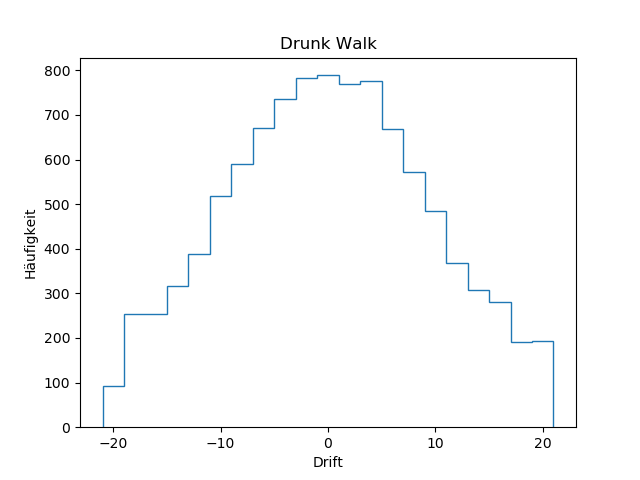
\includegraphics[width=\linewidth]{./gfx/plt-hist-drunkWalk}
	\captionof{figure}{Histogramm zum Drunk Walk}
\end{tcolorbox}
\end{tcbraster}

Für weitere Parameter, siehe \url{https://matplotlib.org/3.1.1/api/_as_gen/matplotlib.axes.Axes.hist.html}

\subsubsection{Vektorfelder}
Die Größen, die wir auftragen wollen, können nicht nur eindimensionale Größen sein, sondern auch eine \enquote{Richtung} haben. Beispielsweise könnten wir Windgeschwindigkeit und -Richtung über einem großen Gebiet darstellen wollen. Zu diesem Zweck dient der Befehl \texttt{quiver}. 

Ähnlich wie schon bei \texttt{plot} und den anderen gezeigten Befehlen reicht es im einfachsten Fall, nur die zu plottenden Daten selbst zu übergeben. Diese müssen dann in \emph{zwei} Listen übergeben werden, da ja auch \emph{zwei}dimensionale Daten dargestellt werden sollen. Die erste Liste enthält also die X-Komponenten der Windrichtungen; in der zweiten Liste sind die Y-Komponenten angegeben. Die Listen selbst müssen dann ebenfalls \emph{zwei}dimensional sein, da die Windgeschwindigkeit an einem \emph{Ort} angegeben wird, der selbst eine X- und Y-Komponente hat.

\begin{codebox}[Beispiel: Wirbelfeld ohne explizite Ortsangabe]
\begin{minted}[linenos]{python3}
import matplotlib.pyplot as plt

width  = 10
height = 15

xPoints = [x / 10 for x in range(- width, + width)]
yPoints = [y / 10 for y in range(-height, +height)]
\end{minted}
\end{codebox}
%
\begin{codebox}[]
\begin{minted}[linenos, firstnumber=last]{python3}
dataX = []
dataY = []

for r, y in enumerate(yPoints) :
    dataX.append([])
    dataY.append([])
    for x in xPoints :
        dataX[r].append(-y)
        dataY[r].append(+x)

plt.quiver(dataX, dataY)
plt.show()
\end{minted}
\end{codebox}

\begin{tcolorbox}[title=Plot: Wirbelfeld]
\begin{center}
	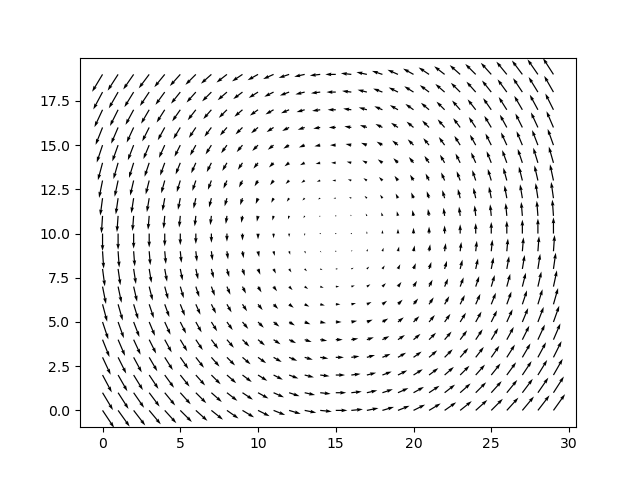
\includegraphics[width=.6\linewidth]{./gfx/plt-vortex}
	\captionof{figure}{Wirbelfeld}
\end{center}
\end{tcolorbox}

\label{ssc:vecFields}
Wie schon zuvor nimmt die MatPlotLib hierzu an, dass die Punkte einen Abstand von 1 zueinander haben, sowohl in X- als auch Y-Richtung. Wo dies nicht der Fall ist, können auch zwei Listen \texttt{X, Y} mit übergeben werden, die jeweils die X- bzw. Y-Koordinate zum \texttt{i}-ten Datenpunkt\footnote{solche Koordinatenlisten können sehr bequem mit der Funktion \texttt{meshgrid} aus dem Modul \texttt{numpy} erstellt werden. Siehe dazu Kapitel \ref{chp:Numpy}}. In diesem Fall dürfen die Listen mit den Pfeil-Daten auch als \emph{eindimensionale} Liste übergeben werden, \ie ihr Index weist ihnen schon ihre Position im Raum zu. Den obigen Plot kann man daher auch mit diesen Zeilen erreichen:

\begin{codebox}[Beispiel: Wirbelfeld ohne explizite Ortsangabe]
\begin{minted}[linenos]{python3}
import matplotlib.pyplot as plt

width  = 10
height = 15
xPoints = [x / 10 for x in range(- width, + width)]
yPoints = [y / 10 for y in range(-height, +height)]
\end{minted}
\end{codebox}
%
\begin{codebox}[]
\begin{minted}[linenos, firstnumber=last]{python3}
X = [xPoints for i in range(2 * height)]
Y = [[y] * 2 * width for y in yPoints]

dataX = []
dataY = []

for y in yPoints :
    for x in xPoints :
        dataX.append(-y)
        dataY.append(+x)

plt.quiver(X, Y, dataX, dataY)
plt.show()
\end{minted}
\end{codebox}

Für weitere Parameter, siehe \url{https://matplotlib.org/3.1.1/api/_as_gen/matplotlib.axes.Axes.quiver.html}

\subsubsection{Weitere Diagrammtypen}
Unter \url{https://matplotlib.org/3.1.0/gallery/index.html} sind diverse Beispiele zum Umgang mit der MatPlotLib aufgeführt.

Beachten Sie auch, dass verschiedene Plot-Typen miteinander vermischt werden können. Ein Balkendiagramm und eine Datenkurve können sich problemlos überlagern.

\section{Multiplots}
Es ist auch möglich, in einem Fenster mehrere Plots darzustellen. Hierzu dienen die Befehle \texttt{subplot} und \texttt{subplots}. Mit \texttt{subplots} wird ein Gitter festgelegt, auf dem die einzelnen Plots im Fenster angeordnet werden. Übergeben werden muss dazu die Anzahl an Zeilen und Spalten, die dieses Gitter haben soll.
\mint{python3}{plt.subplots(2, 4)}
bereitet also ein Fenster vor, in dem insgesamt 8 Plots dargestellt werden können. Diese Plots sind dann in 2 Zeilen und 4 Spalten angeordnet.

Der Befehl \texttt{subplot} wählt aus, an welchen Gitterpunkt der nächste Plot platziert wird. Hierzu ist nochmal die Höhe und Breite des Gitters notwendig; zusätzlich muss auch die \enquote{Nummer des Gitterpunkts} angegeben werden, an die der Plot platziert werden soll. Diese Nummer beginnt bei 1 und wird von links nach rechts und von oben nach unten durchgezählt.
Im oben angelegten 2x4-Gitter wählt also
\mint{python3}{plt.subplot(2, 4, 5)}
den Rasterpunkt in der zweiten Zeile, erste Spalte aus.

Sofern Höhe, Breite und Gitterpunkt-Nummer nur einstellige Ziffern sind, können diese auch zu einer dreistelligen Zahl zusammengefasst werden.
\mint{python3}{plt.subplot(245)}
hat also denselben Effekt, wählt ebenfalls den Rasterpunkt in der zweiten Zeile, erste Spalte aus.

Weiter kann dem Befehl \texttt{subplot} noch über das Keyword-Argument \texttt{polar} ein \inPy{bool}ean mitgegeben werden, der eine Auftragung in Polarkoordinaten verursacht.

\begin{codebox}[Beispiel: Lissajous-Figuren]
\begin{minted}[linenos]{python3}
import math
import matplotlib.pyplot as plt

X = [x / 100 for x in range(628)]
Y = [math.sin(3 * x) for x in X]

plt.subplots(1, 2)
plt.suptitle("Lissajous-Figuren")

plt.subplot(121)
plt.title("Kartesisch")
plt.plot(X, Y)

plt.subplot(122, polar=True)
plt.title("Polarkoordinaten")
plt.plot(X, Y)

plt.show()
\end{minted}
\end{codebox}
%
\begin{tcolorbox}[title=Ausgabe: Lissajous-Figuren]
\begin{center}
	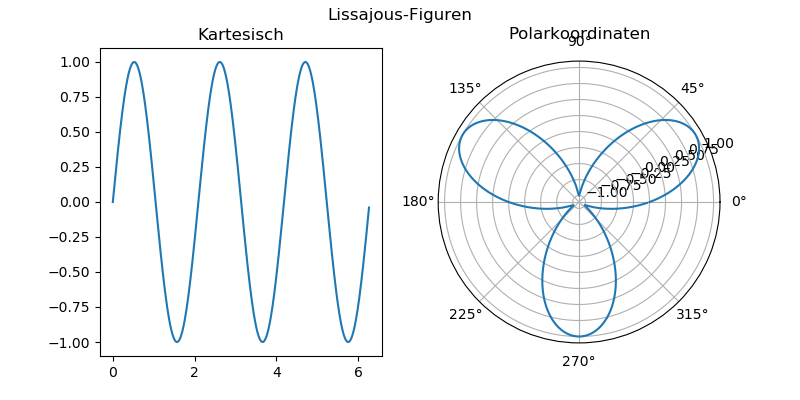
\includegraphics[width=\linewidth]{./gfx/plt-Lissajous}
	\captionof{figure}{Zwei Plots im selben Fenster}
	\label{fig:plt-Lissajous}
\end{center}
\end{tcolorbox}

Siehe \url{https://matplotlib.org/3.3.3/api/_as_gen/matplotlib.pyplot.subplots.html} und \url{https://matplotlib.org/3.3.3/api/_as_gen/matplotlib.pyplot.subplot.html} für weitere Details.

\section{Plot-Objekte}
Wir haben bisher Befehle kennengelernt, die Plots verschiedener Art erstellen und deren Eigenschaften steuern. Im Hintergrund werden hierzu Instanzen von verschiedenen Klassen angelegt. Uns als EntwicklerInnen steht ein solches \emph{objektorientiertes} Herangehen an die Plots auch zur Verfügung: wir können mithilfe der MatPlotLib Objekte erstellen, die die verschiedenen Elemente eines Plots (Fenster, Achsen, Kurven, ...) repräsentieren, und diese Elemente dann über \emph{Methoden} verändern. Dieses Herangehen verlangt eine etwas andere Denkweise, die vielen als natürlicher vorkommt.

Neben diesem Paradigmenwechsel ist es durch die objektorientierte Formulierung von Plots auch möglich, mehrere Plot-Fenster gleichzeitig zu steuern. Außerdem kann Python Code \emph{parallel zum Fenster} ausgeführt werden: normalerweise wird die Code-Ausführung mit \texttt{plt.show()} angehalten, bis das Plot-Fenster geschlossen wird. Im folgenden zeige ich, wie man Python-Code dazu bringt, gleichzeitig zum Betreiben des/der Plot-Fenster(s) weiter den Code auszuführen.

\subsection{Plot-Fenster und \texttt{AxesSubplot}-Objekte}
Bisher haben wir alle Befehle der MatPlotLib direkt über den Alias \texttt{plt} aufgerufen. Tatsächlich werden hierbei verschiedene Instanzen von Klassen angelegt und von der MatPlotLib im Hintergrund verwaltet. Besondere Bedeutung haben dabei die Klassen \texttt{Figure} und \texttt{AxesSubplot}.

Eine \texttt{Figure} stellt ein Plot-Fenster dar. Wir erhalten ein \emph{Handle auf ein neues Fenster} über den Befehl \texttt{figure}:
\mint{python3}{fig = plt.figure()}
Aktionen, die \emph{das Fenster als Ganzes} betreffen, sollten über dieses Handle geschehen.
\mint{python3}{fig.suptitle("Überschrift")}
ändert beispielsweise die Titelzeile des Fensters.

Der Befehl \texttt{figure} hat eine Reihe von Keyword-Parametern, von denen hier nur \texttt{figsize} vorgestellt werden soll. \texttt{figsize} erwartet einen Tupel aus zwei Werten, die die Breite und Höhe des Plots repräsentieren. Für weitere Details, siehe \url{https://matplotlib.org/3.3.3/api/_as_gen/matplotlib.pyplot.figure.html}.

\texttt{AxesSubplot}s repräsentieren die eigentlichen Graphen. Wir erhalten ein Handle auf ein solches Objekt über verschiedene Methoden von \texttt{figure}. Am geläufigsten ist die Methode \texttt{add\_subplot}, die sich im Wesentlichen wie der Befehl \texttt{subplot} verhält:
\mint{python3}{pol = fig.add_subplot(1, 2, 2, projection="polar")}
erzeugt einen Subplot in Polarkoordinaten in der ersten Zeile, zweite Spalte von \texttt{fig}. 
Siehe \url{https://matplotlib.org/3.1.1/api/_as_gen/matplotlib.figure.Figure.html?highlight=add_subplot#matplotlib.figure.Figure.add_subplot} für weitere Details.

Die obige Ausgabe von Abb. \ref{fig:plt-Lissajous} kann so auch mit dem folgenden Code erreicht werden:
\begin{codebox}[Beispiel: Lissajous-Figuren{,} Objektorientiert]
\begin{minted}[linenos]{python3}
import math
import matplotlib.pyplot as plt

X = [x / 100 for x in range(628)]
Y = [math.sin(3 * x) for x in X]

fig = plt.figure(figsize=(8,4))
fig.suptitle("Lissajous-Figuren")

crt = fig.add_subplot(1, 2, 1)
crt.set_title("Kartesisch")
crt.plot(X, Y)

pol = fig.add_subplot(1, 2, 2, projection="polar")
pol.set_title("Polarkoordinaten")
pol.plot(X, Y)

fig.show()

print("Ausgabe noch während der Plot dargestellt wird")
input()
\end{minted}
\end{codebox}

Hier erfolgt die Ausgabe von Zeile 20 schon während der Plot dargestellt wird, und nicht erst, nachdem das Plot-Fenster geschlossen wird. Aus demselben Grund ist auch Zeile 21 notwendig: Der Code läuft nach \texttt{fig.show()} weiter, bis die letzte Zeile ausgeführt wurde; danach beendet Python alle Prozesse, die mit dem Code zu tun hatten, einschließlich der Darstellung des Plots. Mit \inPy{input} zwingen wir Python dazu, auf eine Usereingabe zu warten.

\subsection{Gridspecs}
Erweiterte Kontrolle darüber, wie die Graphen im Plot-Fenster platziert werden, erhalten wir über das \texttt{GridSpec}-Objekt. Dieses ist eine Representation des Gitters, in das die Plots eingetragen werden. Dieses Gitter wird auf das Fenster gelegt, welches wir mit \texttt{plt.figure} angelegt haben; daher auch erhalten wir ein \texttt{GridSpec}-Objekt über eine Methode der Klasse \texttt{figure}. Diese Methode heißt \texttt{add\_gridspec} und erwartet zwei \inPy{int}-Werte, die die Anzahl der Zeilen und Spalten im Gitter darstellen -- also dieselben Werte, wie wir sie schon von \texttt{subplots} bzw. \texttt{subplot} kennen.

Der Rückgabewert von \texttt{add\_gridspec} ist ein Array-artiges Objekt, \ie wir können die einzelenen Zellen des Gitters über Indices in eckigen Klammern ansprechen. Auch Slicing ist möglich, um zusammenhängende Bereiche auszuzeichnen. Wenn \texttt{gs} das \texttt{GridSpec}-Objekt ist, dann ist \texttt{gs[1, 0]} die Zelle in der zweiten Zeile, erste Spalte; \texttt{gs[:, 2]} stellt die \emph{gesamte} dritte Spalte dar.

Dieses \texttt{GridSpec}-Objekt kann auch an \texttt{add\_subplot} übergeben werden, und legt wieder fest, wo im Fenster as zugehörige \texttt{AxisSubplot}-Objekt platziert werden soll.

Wenn zwei Graphen \enquote{verwandte} Daten darstellen sollen, wollen Sie vielleicht auch, dass die Skalierung der Achsen in beiden Graphen gleich sind. Dies erreichen Sie durch die Keyword-Arguments \texttt{sharex} und \texttt{sharey} in \texttt{add\_subplot}. Diesen wird jeweils das \texttt{AxisSubplot}-Objekt übergeben, an das die X- bzw. Y-Achse gekoppelt werden soll.

Das folgende Beispiel nutzt ein \texttt{GridSpec}-Objekt, um einen großen Plot und zwei kleinere Plots anzuordnen. Nicht alle hierin verwendeten Methoden der MatPlotLib wurden bereits besprochen; sicher aber können Sie sich aus dem Kontext erschließen, welchen Zweck diese Stellen erfüllen\footnote{Die MatPlotLib bringt eine gewaltige Fülle an Funktionen mit, die kaum zu überblicken oder im Kopf zu behalten ist. In der Praxis heißt die Arbeit mit de MatPlotLib oft, im Internet nach Beispieln zu suchen, und aus den dort gezeigten Code-Schnipseln die Stellen zu isolieren, die das gesuchte Feature aktivieren. Sie üben hier also eine Kernkompetenz des Programmierens: unbekannten Code zu interpretieren. Kopieren Sie den Code und experimentieren Sie mit den Einstellungen, um tiefere Einblicke zu gewinnen! Sie können auch immer die QuickSearch-Funktion auf \url{https://matplotlib.org/3.1.1/index.html} zur Hilfe nehmen.}.

\begin{codebox}[Beispiel: 2D-Normalverteilung]
\begin{minted}[linenos]{python3}
import random
import matplotlib.pyplot as plt

N      = 1000
X      =   50
Y      =   40
sigmaX =    5
sigmaY =   10

dataX = [random.gauss(X, sigmaX) for _ in range(N)]
dataY = [random.gauss(Y, sigmaY) for _ in range(N)]

fig = plt.figure(figsize=(8,8))
gs  = fig.add_gridspec(3, 3)

fig.suptitle("2D-Normalverteilung")
fig.subplots_adjust(wspace=0.2, hspace=0.3)

axScatter = fig.add_subplot(gs[0:2, 0:2])
axScatter.set_xlim(0, 100)
axScatter.set_ylim(0, 100)
axScatter.set_xlabel("x")

axHistX   = fig.add_subplot(gs[ 2 , 0:2], sharex=axScatter)
axHistY   = fig.add_subplot(gs[0:2,  2 ], sharey=axScatter)

axScatter.scatter(dataX, dataY, marker=".")
axHistX.hist(dataX, orientation='vertical'  , bins=20)
axHistY.hist(dataY, orientation='horizontal', bins=20)

fig.show()
input()
\end{minted}
\end{codebox}
%
\begin{tcolorbox}[title=Ausgabe: 2D-Normalverteilung]
\begin{center}
	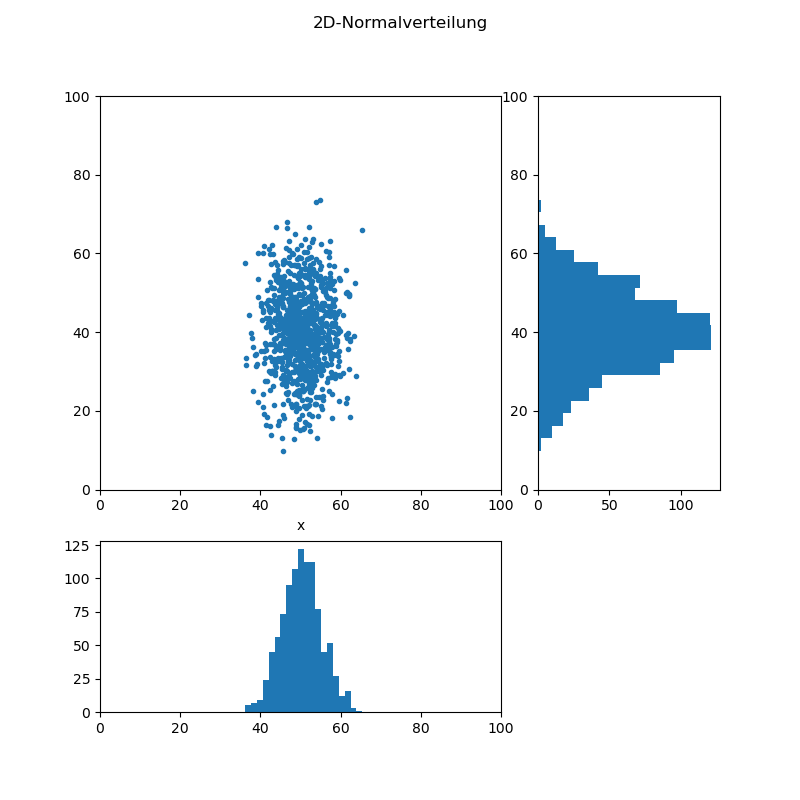
\includegraphics[width=.7\linewidth]{./gfx/plt-gauss2D}
	\captionof{figure}{Komplexere Anordnung von Plots: 2D-Normalverteilung}
\end{center}
\end{tcolorbox}


\subsection{Manipulation des \texttt{AxisSubplot}-Objekts}
Wie Sie sich schon aus dem letzten Beispiel erschlossen haben, können mit \texttt{set\_xlim}, \texttt{set\_ylim} die Grenzen festgelegt werden, auf die die X- bzw. Y-Achse skaliert werden. In ähnlicher Weise dienen die Befehle \texttt{set\_title}, \texttt{set\_xlabel}, \texttt{set\_ylabel}, \texttt{set\_xscale} und \texttt{set\_yscale} dazu, Überschrift des Graphen, Achsenbeschriftung und Auftragung (linear, logarithmisch, ...) zu bestimmen. Alle diese Methoden können auf ein \texttt{AxisSubplot}-Objekt angewandt werden.

\begin{hintbox}[Getter und Setter]
Ebenso wie es mit \texttt{set\_XXX} möglich ist, den Wert \texttt{XXX} eines \texttt{AxisSubplot}-Objekts festzulegen, kann mit \texttt{get\_XXX} der aktuell eingespeicherte Wert abgefragt werden. Dies ist eine gängige Praxis in der objektorientierten Programmierung: Wenn eine Klasse ein Attribut \texttt{XXX} hat, so sollte es hierzu auch die Methoden \texttt{get\_XXX} und \texttt{set\_XXX} geben.

Wir werden auf solche Design-Pattern in Kaptiel \ref{chp:Classes2} nochmals eingehen.
\end{hintbox}

Die Bemaßung eines \texttt{AxisSubplot}-Objekts \texttt{ax} kann auch mit \texttt{ax.axis} gesetzt bzw. abgefragt werden.
\begin{tabular}{p{.4\linewidth}p{.1\linewidth}c}
\inPy{xmin, xmax = ax.get_xlim()} & \multirow{2}{*}{bzw.}  & \inPy{ax.set_xlim(xmin, xmax)} \\
\inPy{ymin, ymax = ax.get_ylim()} &      & \inPy{ax.set_ylim(ymin, ymax)}
\end{tabular}

sind also äquivalent zu\\
\begin{tabular}{p{.4\linewidth}p{.1\linewidth}c}
\inPy{xmin, xmax, ymin, ymax = ax.axis()} & bzw. & \inPy{ax.axis(xmin, xmax, ymin, ymax)}
\end{tabular}.

Zusätzlich erlaubt die Methode \texttt{axis} auch, die Achsen eines Graphen komplett zu verbergen (\inPy{ax.axis("off")}), so zu skalieren dass gleiche Abstände in X- und Y-Richtung auch gleichen Skalenschritten entsprechen (\inPy{ax.axis("equal")}), oder dass die Graphen-Fläche zu einem Quadrat verzerrt wird (\inPy{ax.axis("square")}). Siehe hierzu auch \url{https://matplotlib.org/3.1.1/api/_as_gen/matplotlib.axes.Axes.axis.html#matplotlib.axes.Axes.axis}.

Über \texttt{set\_xtics} und \texttt{set\_ytics} lässt sich einstellen, an welchen Punkten die X- bzw. Y-Achse unterteilt werden sollen. Wir unterscheiden hierbei \emph{major ticks} (größere Abstände und längere Striche, \idR mit Zahlenwert) und \emph{minor ticks} (kleinere Abstände, kurzere Striche, \idR ohne Zahlenwert). Übergeben werden hierfür verpflichtend eine \inPy{list} mit den Zahlenwerten, an denen Ticks gesetzt werden sollen. Das Optionale Schlüsselwort \texttt{minor} kann entweder auf \inPy{True} oder \inPy{False} gesetzt werden; entsprechend gilt die Liste der Ticks dann auch für die \emph{minor} oder \emph{major} Ticks.

\begin{codebox}[Beispiel: Major- und Minor Ticks, width=.55\linewidth, nobeforeafter, equal height group = grpXmpSimpleTicks]
\begin{minted}[linenos]{python3}
import matplotlib.pyplot as plt

fig = plt.figure(figsize=(6,2))
gfx = fig.subplots()

xMajor = [10 / x    for x in range(1,  5)]
xMinor = [5 + x / 2 for x in range(1, 10)]

gfx.set_xticks(xMajor)
gfx.set_xticks(xMinor, True)

plt.show()
\end{minted}
\end{codebox}
%
\begin{tcolorbox}[title=Ausgabe: Major- und Minor Ticks, width=.45\linewidth, nobeforeafter, equal height group = grpXmpSimpleTicks]
	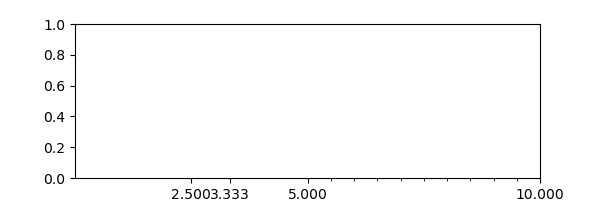
\includegraphics[width=\linewidth]{./gfx/plt-ticks}
	\captionof{figure}{Major- und Minor Ticks}
	Man beachte die kleinen Unterteilungen zwischen 5.0 und 10.0 (minor ticks)
\end{tcolorbox}

Siehe auch \url{https://matplotlib.org/3.1.1/api/_as_gen/matplotlib.axes.Axes.grid.html#matplotlib.axes.Axes.grid} für Methoden zur Beeinflussung der Gitternetzlinien.

\subsection{Ticker}
Wir können nicht nur beeinflussen, welche Werte an den Achsen durch Ticks markiert sein sollen, sondern auch, welche Beschriftungen dort stehen sollen. Im einfachsten Fall können wir einfach direkt eine Liste von Texten vorgeben. Hierzu dienen die Befehle \texttt{set\_xticklabels} und \texttt{set\_yticklabels}. \emph{Verpflichtend} muss eine \inPy{list} von Strings übergeben werden, die nacheinander an der X- bzw. Y-Achse angetragen werden sollen. Der erste Wert der Liste wird an den ersten Tick gesetzt, der Zweite an den Zweiten, etc.

Weiter gibt es die optionalen Keyword-Arguments \texttt{minor} und \texttt{fontdict}. Wie schon bei \texttt{set\_xtics} / \texttt{set\_ytics} ist \texttt{minor} ein \inPy{bool} und dient der Zuordnung zu den Major- oder Minor Ticks. Standardmäßig ist dieses Argument \inPy{False}, \ie man beschreibt die Major Ticks.

Wie es der Name vermuten lässt, ist \texttt{fontdict} ein \inPy{dict}, in dem Einstellungen zur Schriftart enthalten sind.

Beispiel:
\begin{minted}{python3}
ax.set_xticklabels(
    ['Bill', 'Fred', 'Mary', 'Sue'],
    fontdict={'fontsize' :15, 'fontweight' : 'bold'}
)
\end{minted}
weist der X-Achse die vier Labels \texttt{'Bill'}, \texttt{'Fred'}, \texttt{'Mary'} und \texttt{'Sue'} zu. Diese werden In Schriftgröße 15 in Fettdruck gerendert.

Siehe \url{https://matplotlib.org/3.3.3/api/_as_gen/matplotlib.axes.Axes.set_xticklabels.html} für weitere Details.

Wo mehr Flexibilität nötig ist, kann das Modul \texttt{matplotlib.ticker} verwendet werden. Dieses stellt mehrere Methoden zur Verfügung, wie automatisiert Beschriftungen aus den Achsenwerten generiert werden können. Besonders praktisch ist hierbei die Idee eines \emph{FuncFormatters}: Hierbei handelt es sich um eine benutzerdefinierte Funktion, die aus dem Achsenwert eine vollständige Beschreibung (Text, Schriftart, Position, ...) der Beschriftung generiert. Einen solcher FuncFormatter erhalten wir, indem wir
\begin{itemize}
\item eine Funktion schreiben, die aus einem Zahlenwert den Text für die Beschriftung erzeugt.
	\begin{itemize}
	\item Die Funktion muss zwei Parameter annehmen: Wert auf der Achse und Tick-Nummer
	\item Der Rückgabetyp der Funktion muss ein String sein.
	\end{itemize}
\item diese Funktion an \texttt{matplotlib.ticker.FuncFormatter} übergeben.
\end{itemize}
Ein solches \texttt{FuncFormatter}-Objekt kann dann an \texttt{ax.xaxis.set\_major\_formatter}, \texttt{ax.xaxis.set\_minor\_formatter}, \texttt{ax.yaxis.set\_major\_formatter} oder  \texttt{ax.yaxis.set\_minor\_formatter} übergeben werden.


\begin{codebox}[Beispiel: FuncFormatter für Y-Ticks]
\begin{minted}[linenos]{python3}
from matplotlib.ticker import FuncFormatter
import matplotlib.pyplot as plt

x = list(range(4))
money = [1.5e5, 2.5e6, 5.5e6, 2.0e7]

# Der Plot selbst
fig = plt.figure(figsize=(7,4))
ax = fig.subplots()
ax.bar(x, money)

# Beschriftung der X-Achse
ax.set_xticks(x)
ax.set_xticklabels(
  ['Bill', 'Fred', 'Mary', 'Sue'],
  fontdict={'fontsize' :15, 'fontweight' : 'bold'}
)

# Beschriftung der Y-Achse
def myTicks(x, pos):
    return f"{(x * 1e-6):1.1f}M, #{pos}"


formatter = FuncFormatter(myTicks)
print(formatter)
ax.yaxis.set_major_formatter(formatter)

plt.show()
\end{minted}
\end{codebox}
%
\begin{tcolorbox}[title=Ausgabe: FuncFormatter für Y-Ticks]
\begin{center}
	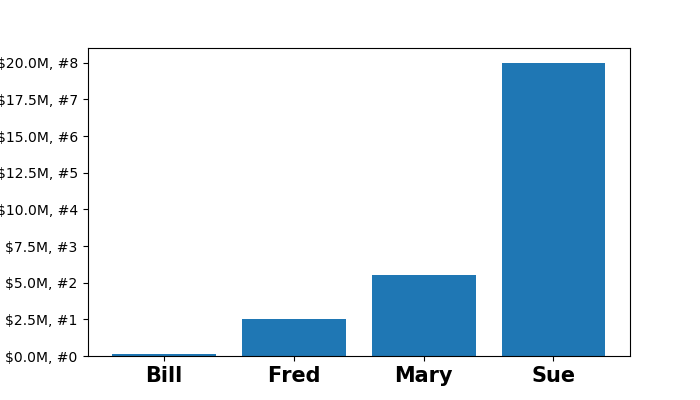
\includegraphics[width=.7\linewidth]{./gfx/plt-TicksFormatter}
	\captionof{figure}{Major- und Minor Ticks}
\end{center}
\end{tcolorbox}

Siehe hierzu auch \url{https://matplotlib.org/3.1.1/gallery/ticks_and_spines/tick-formatters.html} für Beispiele.


\subsection{\LaTeX-Elemente in Plots}
Python enthält ein eigenständiges \LaTeX-Modul, das zur Darstellung von einfachen mathematischen Gleichungen geeignet ist. Um Teile eines Strings als \LaTeX-Code zu interpretieren, können diese einfach durch Dollarzeichen \texttt{\$} eingerahmt werden. So führt beispielsweise
\begin{center}
\inPy{plt.title(r"$\frac{\pi}{2} \approx$ 3.1415")}
\end{center}
zu der Ausgabe
\[ \scriptstyle \frac{\pi}{2} \approx \text{3.1415} \]

\begin{hintbox}[Escaping Unterbinden: R-Strings]
Befehle in \LaTeX beginnen mit einem Backslash (\textbackslash). In Python wird der Backslash in Strings als Escape-Zeichen interpretiert, \ie nachfolgende Zeichen werden anders interpretiert, \eg \texttt{\textbackslash n} für einen Zeilenumbruch. Um dies zu unterbinden kann einem String ein \texttt{r} vorangestellt werden, wie im obigen Beispiel gezeigt.
\end{hintbox}

Die MatPlotLib verwaltet eine ganze Reihe von Standard-Einstellungen. Diese sind in einem \inPy{dict} namens \texttt{matplotlib.rcparams} gespeichert und können zu jeder Zeit geändert werden. Die Schlüssel des \inPy{dict}s sind einfache Strings. Soll für aufwändigere \LaTeX-Elemente nicht das Python-Backend für \LaTeX benutzt werden sondern ein bereits auf dem Rechner vorliegender \LaTeX-Compiler genutzt werden, so kann dies über den \inPy{dict}-Eintrag \texttt{text.usetex} geschehen. Zugeordnet ist ein \inPy{bool}, der festlegt, ob Labeltexte generell als \LaTeX-Code Interpretiert werden sollen. 

Indem wir also die Zeilen
\begin{minted}{python3}
import matplotlib
matplotlib.rcParams['text.usetex'] = True
\end{minted}
zu unserem Plot hinzufügen, können wir sehr einfach professionell aussehende Labels erzeugen und auch Formel-Elemente einfügen:

\begin{codebox}[Beispiel: Mathematisches Pendel mit \LaTeX-Elementen]
\begin{minted}[linenos]{python3}
import math
import matplotlib
matplotlib.rcParams['text.usetex'] = True
import matplotlib.pyplot as plt

T = [x / 100 for x in range(100)]
S = [math.cos(4 * math.pi * t) + 2 for t in T]

plt.plot(T, S)
plt.xlabel(r'\textbf{time (s)}')
plt.ylabel('\\textit{Velocity (\N{DEGREE SIGN}/sec)}', fontsize=16)
plt.title (r'\TeX\ is Number $\displaystyle\sum_{n=1}^\infty'
           r'\frac{-e^{i\pi}}{2^n}$!', fontsize=16, color='r')
plt.show()
\end{minted}
\end{codebox}
%
\begin{tcolorbox}[title=Ausgabe: Mathematisches Pendel mit \LaTeX-Elementen]
\begin{center}
	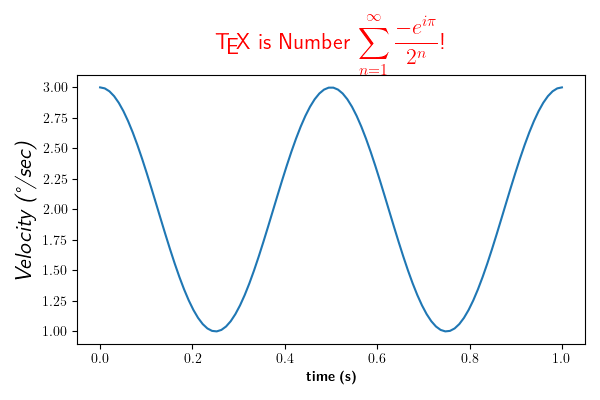
\includegraphics[width=.7\linewidth]{./gfx/plt-tex}
	\captionof{figure}{\LaTeX-Elemente im Plot}
\end{center}
\end{tcolorbox}

\begin{hintbox}[Fehlende Komponenten Nachinstallieren]
Wenn Sie die Beispiele aus diesem Abschnitt ausführen, erhalten Sie möglicherweise die Fehlermeldung\\
\emph{RuntimeError: Failed to process string with tex because dvipng could not be found}\\
oder ähnliche Hinweise auf fehlende Komponenten.

Bei der empfohlenen Anaconda-Installation kann das Python-eigene LaTeX-Modul aus der Anacona-Konsole heraus nachinstalliert werden mit:\\
\texttt{pip install latex}\\
Linux-UserInnen geben diesen Befehl in die normale Konsole ein (ggf. mit \texttt{sudo}).

Für das Beispiel \emph{Mathematisches Pendel mit \LaTeX-Elementen} muss ein \LaTeX-Compiler installiert sein. Als Linux-UserIn können Sie die Komponenten nachinstallieren mit dem Konsolen-Befehl:\\
\texttt{sudo apt install texlive texlive-latex-extra texlive-fonts-recommended dvipng}\\
Beachten Sie, dass die Installation lange dauern kann und nennenswert Festplattenspeicher beansprucht.

Windows- und Mac-UserInnen halten sich hierfür am besten an die Standard-Installation, wie von der TeX Live Website \url{https://www.tug.org/texlive/} angeboten.
\end{hintbox}

Siehe auch \url{https://matplotlib.org/3.3.3/tutorials/introductory/customizing.html?highlight=text.usetex#matplotlib-rcparams} und \url{https://matplotlib.org/3.3.3/gallery/text_labels_and_annotations/tex_demo.html#sphx-glr-gallery-text-labels-and-annotations-tex-demo-py} für weitere Details.

\subsection{Rückgabewerte der Plot-Funktionen}
Bei den Histogrammen haben wir schon gesehen, dass auch die Plot-Befehle selbst (\texttt{plot}, \texttt{bar}, \texttt{hist}, ...) Rückgabewerte haben können. Die Rückgabeobjekte sind im Detail jeweils verschieden; allen gemein ist jedoch, dass sie die Gesamtheit der gezeichneten Objekte repräsentieren.

Wir wollen hier zumindest auf den Rückgabewert von \texttt{plot} näher eingehen; von hier können Sie hoffentlich Analogien auf die anderen Objekte bilden, die Ihnen bei der Arbeit mit der MatPlotLib begegnen können.

Beginnen wir mit einem Code zur Analyse:
\begin{codebox}[Beispiel: Rückgabewerte von \texttt{plt.plot}]
\begin{minted}[linenos]{python3}
import math
import matplotlib.pyplot as plt

X = [x / 100 for x in range(0, 628, 5)]
Y = [math.sin(2 * t) + 2 for t in X]

p = plt.plot(X, Y, "y-", label="foo")
q = plt.plot(X, Y, "r.", label="bar")

print(type(p), p[0], type(p[0]))
print(type(q), q[0], type(q[0]))
\end{minted}
\end{codebox}
%
\begin{cmdbox}[Ausgabe: Rückgabewerte von \texttt{plt.plot}]
\begin{minted}{text}
<class 'list'> Line2D(foo) <class 'matplotlib.lines.Line2D'>
<class 'list'> Line2D(bar) <class 'matplotlib.lines.Line2D'>
\end{minted}
\end{cmdbox}

Wir sehen, dass der Rückgabewert von \texttt{plot} eine \inPy{list} von Instanzen der Klasse \texttt{matplotlib.lines.Line2D} ist. Jede solche Instanz repräsentiert nun wie erwähnt eine Linie des Graphen, \ie enthält die Werte der Datenpunkte sowie die von uns explizit und implizit zugewiesenen Formatierungen (\eg Name der Datenreihe \texttt{foo} bzw. \texttt{bar}, oder \emph{Linienfarbe blau}). Wenn wir nun die zugehörige Seite der Dokumentation der MatPlotLib aufrufen (\url{https://matplotlib.org/3.1.1/api/_as_gen/matplotlib.lines.Line2D.html}), finden wir eine große Zahl von Methoden, die auf dieses Objekt angewandt werden können, sowie eine kurze Erläuterung, welchen Zweck diese Methoden erfüllen, und welche Parameter erwartet werden.

Ein Anwendungszweck ist die Nutzung mit \texttt{legend}. Wie Sie wissen, sorgt \texttt{legend} dafür, dass die Legende zu einem Plot angezeigt wird. Im obigen Beispiel wird ein Plot vorbereitet, bei dem derselbe Datensatz einmal mit einer gelben Linie und einemal mit roten Punkten dargestellt wird. Würden wir hier direkt mit \texttt{plt.legend()} eine Legende erzeugen, so hätte diese auch zwei Einträge.

Um in einem solchen Fall den unnötigen Legendeneintrag zu unterdrücken, können wir dem Befehl \texttt{legend} zwei \inPy{list}s mitgeben. Die erste solche \inPy{list} enthält alle Handles auf darzustellende Linien (also alle \texttt{matplotlib.lines.Line2D}-Objekte); in die zweite \inPy{list} schreiben wir alle Legendeneinträge.

\begin{codebox}[Beispiel: Legendeneinträge unterdrücken, width=.55\linewidth, nobeforeafter, equal height group = grpXmpLegendSelect]
\begin{minted}[linenos]{python3}
import math
import matplotlib.pyplot as plt

X = [x / 100 for x in range(0, 628, 5)]
Y = [math.sin(2 * t) + 2 for t in X]

fig = plt.figure()
drw = fig.subplots()

p = drw.plot(X, Y, "y-", label="foo")
q = drw.plot(X, Y, "r.", label="bar")

drw.legend(p, ["FOOBAR"])
plt.show()
\end{minted}
\end{codebox}
%
\begin{tcolorbox}[title=Legendeneinträge unterdrücken, width=.45\linewidth, nobeforeafter, equal height group = grpXmpLegendSelect]
\begin{center}
	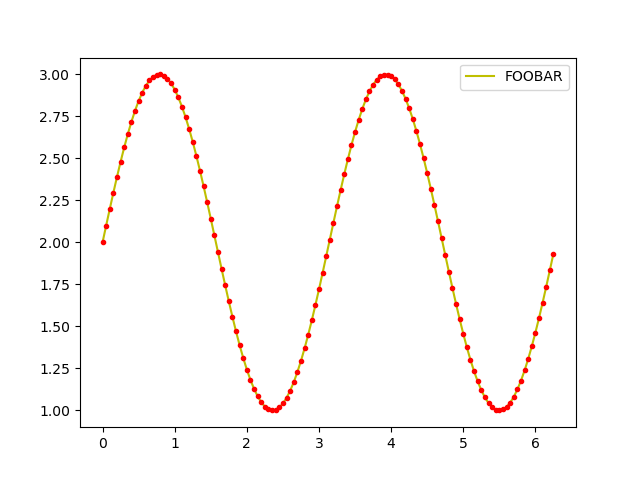
\includegraphics[width=\linewidth]{./gfx/plt-legend-select}
	\captionof{figure}{Legendeneinträge unterdrücken}
\end{center}
\end{tcolorbox}

\subsection{Text und Overlays}
In ein Plotfenster können beliebige Zeichen- und Textelemente hinzugefügt werden. Hier soll nur gezeigt werden, wie Sie Textanmerkungen und Pfeile auf einem Plot anbringen. Für andere Elemente, siehe \url{https://matplotlib.org/3.1.1/gallery/text_labels_and_annotations/annotation_demo.html#sphx-glr-gallery-text-labels-and-annotations-annotation-demo-py}

Texte platzieren Sie in Ihrem Plot mit dem Befehl \texttt{annotate}. Hierzu müssen Sie angeben welcher Text geschrieben werden soll und an welchen Koordinaten er im Plot erscheinen soll; letzteres wird über den Schlüsselwort-Parameter \texttt{xy} als \inPy{tuple} angegeben. In seiner Minimalform lautet der Befehl dann also:
\mint{python3}{ax.annotate("text", xy=(x, y))}
wobei \texttt{x, y} im Koordinatensystem des Plots sind.

\begin{codebox}[Beispiel: Plot mit Text-Overlay, width=.55\linewidth, nobeforeafter, equal height group = grpXmpSimpleOverlay]
\begin{minted}[linenos]{python3}
import math
import matplotlib.pyplot as plt

X = [x / 100 for x in range(0, 628, 5)]
Y = [math.sin(t) for t in X]

fig = plt.figure()
drw = fig.subplots()

drw.plot(X, Y)

drw.annotate("Die Sinus-Funktion,\n"     +
             "wie von der math-library\n"+
             "zur Verfügung gestellt",
             xy=(3.5, 0.5)
)
plt.show()
\end{minted}
\end{codebox}
%
\begin{tcolorbox}[title=Ausgabe: Plot mit Text-Overlay, width=.45\linewidth, nobeforeafter, equal height group = grpXmpSimpleOverlay]
	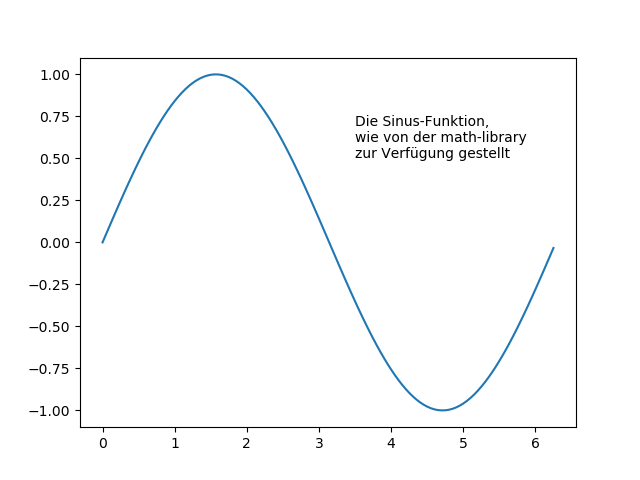
\includegraphics[width=\linewidth]{./gfx/plt-overlay-simple}
	\captionof{figure}{Plot mit Text-Overlay}
\end{tcolorbox}

Manchmal ist es günstiger, die Koordinaten des Textfeldes nicht bezüglich des Plotfensters anzugeben, sondern ein anderes Koordinatensystem zu wählen. Andere mögliche Referenzpunkte können über den optionalen Paremeter \texttt{xycoords} festgelegt werden. Diesem wird einer der folgenden Strings zugewiesen:
\begin{center}
\begin{tabular}{m{0.3\linewidth}m{0.6\linewidth}}
	\textbf{String}          & \textbf{Wirkung} \tabcrlf
	\inPy{'figure points'}   & Abstand vom linken oberen Rand des Plot-Fenstes in Punkten \\
	\inPy{'figure pixels'}   & Abstand vom linken oberen Rand des Plot-Fenstes in Pixeln \\
	\inPy{'figure fraction'} & Abstand vom linken oberen Rand des Plot-Fenstes als Bruch der Gesamtbreite, 
	                           \ie \inPy{(0,0)} steht für die linke untere Ecke und \inPy{(1,1)} für doe rechte obere Ecke\\
	\inPy{'axes points'}     & Abstand vom Koordinatenursprung des Plots in Punkten\\
	\inPy{'axes pixels'}     & Abstand vom Koordinatenursprung des Plots in Pixeln\\
	\inPy{'data'}            & Koordinaten wie durch den Graphen definiert (default)\\
\end{tabular}
\captionof{table}{Mögliche Koordinatenursprünge für \texttt{xycoords} in \texttt{ax.annotate}}
\label{tab:plt.annotate.xycoords}
\end{center}

Die Orientierung des Texts bezüglich des angegebenen Punkts kann weiter mit den optionalen Parametern \texttt{horizontalalignment} und \texttt{verticalalignment} gesteuert werden:
\begin{center}
\begin{tabular}{cc}
	\textbf{Parameter}           & \textbf{erlaubte Werte} \tabcrlf
	\texttt{horizontalalignment} & \inPy{'left'}, \inPy{'center'}, \inPy{'right'} \\
	\texttt{verticalalignment}   & \inPy{'top'}, \inPy{'center'}, \inPy{'bottom'}
\end{tabular}
\captionof{table}{Mögliche Alignments für \texttt{ax.annotate}}
\end{center}

Schließlich ist es auch möglich, mit dem Text auf einen bestimmten Aspekt im Plot hinzuweisen. Hierzu benutzen wir die optionalen Parameter \texttt{arrowprops}, \texttt{textxy} und \texttt{textcoords}.

Da wir nun zwei Dinge platzieren müssen -- Text und Pfeilspitze -- haben wir ein zusätzliches Koordinatenpaar \texttt{textxy}, das an die Stelle von \texttt{xy} im einfachen Fall tritt. D.\;h. die Pfeilspitze wird durch \texttt{xy} ausgezeichnet, während die Text-Koordinaten durch \texttt{textxy} beschrieben werden. Für \texttt{textcoords} gilt dasselbe, was schon zu \texttt{xycoords} gesagt wurde, \ie es handelt sich um Werte aus Tabelle \ref{tab:plt.annotate.xycoords}. Zusätzlich sind auch noch diese Werte möglich:
\begin{center}
\begin{tabular}{m{0.3\linewidth}m{0.6\linewidth}}
	\textbf{String}          & \textbf{Wirkung} \tabcrlf
	\inPy{'offset points'}   & Koordinaten relativ zu \texttt{xy} in Punkten\\
	\inPy{'offset pixels'}   & Koordinaten relativ zu \texttt{xy} in Pixeln\\
\end{tabular}
\captionof{table}{Zusätzlich mögliche Koordinatenursprünge für \texttt{textcoords} in \texttt{ax.annotate}}
\end{center}
Weiterhin beziehen sich \texttt{horizontalalignment} und \texttt{verticalalignment} auf die Ausrichtung des Texts.

Schließlich legt \texttt{arrowprops} fest, wie der Pfeil aussehen soll. Es handelt sich um ein \inPy{dict}, in dem verschiedene Schlüssel-Wert-Paare den Pfeil beschreiben. Eine (unvollständige!) Auswahl von möglichen Paaren finden Sie hier:
\begin{center}
\begin{tabular}{m{.15\linewidth}m{.15\linewidth}m{.4\linewidth}m{.15\linewidth}}
	\textbf{Schlüssel} & \textbf{Wert}                     & \textbf{Wirkung}        & \textbf{Default} \tabcrlf
	\inPy{'facecolor'} & (ein Farbwert) oder \inPy{'none'} & Füllfarbe des Pfeils    & Standard-Blau    \\
	\inPy{'edgecolor'} & (ein Farbwert) oder \inPy{'none'} & Randfarbe des Pfeils    & \inPy{'black'}   \\
	\inPy{'color'}     & (ein Farbwert)                    & Rand- und Füllfarbe des
	                                                         Strings (überschreibt
	                                                         \texttt{facecolor} und
	                                                         \texttt{edgecolor})     & (nicht gesetzt)  \\
	\inPy{'shrink'}   & (Zahl zwischen 0 und 1)            & Verkürzt den Pfeil um 
	                                                         angegebenen Faktor      & 1                \\
  \inPy{'width'}    & (Zahl)                             & Breite des Pfeils in 
                                                           Punkten                 & 4                \\
  \inPy{'frac'}\\
  \inPy{'headwidth'}& (Zahl)                             & Breite der Pfeilspitze
                                                           in Punkte               & 10
\end{tabular}
\captionof{table}{Mögliche Schlüssel-Wert-Paare für \texttt{arrowprops} in \texttt{ax.annotate}}
\end{center}

Die Beispiele auf \url{https://matplotlib.org/3.1.1/gallery/text_labels_and_annotations/annotation_demo.html#sphx-glr-gallery-text-labels-and-annotations-annotation-demo-py} zeigen Ihnen weitere Einstellmöglichkeiten. Siehe auch \url{https://matplotlib.org/3.1.1/api/_as_gen/matplotlib.axes.Axes.annotate.html#matplotlib.axes.Axes.annotate} für weitere Details.

\section{3D-Plots}
Auf einem zweidimensionalen Bildschirm (oder Ausdruck) kann natürlich nur eine zweidimensionale Projektion eines dreidimensionalen Objekts dargestellt werden. Dies schränkt die \emph{Lesbarkeit} bzw. wissenschaftliche Verwertbarkeit von Visualisierungen von Daten ein; dafür erlauben Sie eine sehr viel intuitivere Wahrnehmung eines Sachverhalts. Und nicht zuletzt, 3D-Bilder sehen einfach \emph{cool} aus.

Die MatPlotLib hält natürlich auch hierzu Methoden bereit. Wir wollen hier also auch einige Features der MatPlotLib ansprechen. Ein ausführlicheres Tutorial finden Sie unter \url{https://matplotlib.org/mpl_toolkits/mplot3d/tutorial.html}.

\subsection{Das \texttt{Axes3D}-Objekt}
\begin{minipage}{\linewidth}
Die Darstellung von 3D-Daten wird von einem eigenen Teil der MatPlotLib-Library geleistet, der zuerst in unser Projekt geladen werden muss. Dies geschieht über die Zeile:
\vspace{-6pt}
\begin{center}
	\inPy{from mpl_toolkits.mplot3d import Axes3D}
\end{center}
\end{minipage}

Mit dieser Ergänzung können wir ein \texttt{Axes3D}-Objekt erzeugen, auf dem unsere 3D-Ausgaben erfolgen. Dieses Objekt erhalten wir über die Methode \texttt{add\_subplot}, die wir bereits kennengelernt haben. Zusätzlich zu den früheren Aufrufen können wir jetzt den optionalen Parameter \inPy{projection='3d'} übergeben.

\begin{codebox}[Beispiel: Leerer 3D-Plot, width=.55\linewidth, nobeforeafter, equal height group = grpXmpEmpty3D]
\begin{minted}[linenos]{python3}
import matplotlib.pyplot as plt
from mpl_toolkits.mplot3d import Axes3D

fig = plt.figure()
drw = fig.add_subplot(projection='3d')

plt.show()
\end{minted}
\end{codebox}
%
\begin{tcolorbox}[title=Ausgabe: Leerer 3D-Plot, width=.45\linewidth, nobeforeafter, equal height group = grpXmpEmpty3D]
	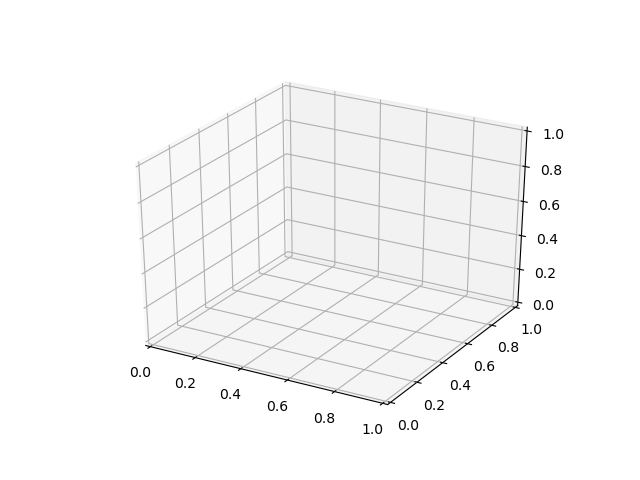
\includegraphics[width=\linewidth]{./gfx/plt-axes3D}
	\captionof{figure}{Leerer 3D-Plot}
\end{tcolorbox}

Auf dieses \texttt{Axes3D}-Objekt können nun die bereits bekannten Methoden zum erstellen von Plots angewandt werden. Natürlich erwarten diese jetzt nicht nur Listen von X- und Y-Koordinaten, sondern auch die zugehörigen Z-Koordinaten. Grundsätzlich aber bleibt das Herangehen das Ihnen bereits bekannte. Im weiteren soll dies an zwei Beispielen genauer gezeigt werden.

\subsection{Kurven im Raum}
Sobald ein \texttt{Axes3D}-Objekt initialisiert wurde, kann die Methode \texttt{plot} wie gewohnt eingesetzt werden. Verlangt werden jetzt \emph{3} Parameter, die die X- Y- und Z-Koordinaten enthalten. Ansonsten gelten die oben besprochenen Techniken weiter.

Einstellungen, die die dritte Achse betreffen, können über dieselben Methoden geleistet werden, die die ersten beiden Achsen betreffen, indem das \texttt{x} bzw. \texttt{y} durch ein \texttt{z} ersetzt wird. Die Achsenbeschriftung können wir beispielsweise durch \texttt{set\_zlabel} ändern.

Um die Ansicht zu drehen kann der Befehl \texttt{view\_init} benutzt werden. Dieser erwartet zwei Zahlen, die die Raumwinkel darstellen, in dem der Plot betrachtet wird. Die erste Zahl ist hierbei die \emph{Inklination}, also wie steil \enquote{die Kamera} auf den Plot gerichtet ist; die zweite Zahl dagegen ist die \emph{Deklination}, also die Drehung in der X-Y-Ebene. Experimentieren Sie im Zweifel herum, um die für Sie geeigneten Einstellungen zu finden.

\begin{codebox}[Beispiel: 3D-Kurve]
\begin{minted}[linenos]{python3}
import math
import matplotlib.pyplot as plt
from mpl_toolkits.mplot3d import Axes3D

fig = plt.figure()
drw = fig.add_subplot(projection='3d')

T = [math.pi * t / 100 for t in range(1000)]
X = [math.exp(-0.05 * t) * math.cos(t) for t in T]
Y = [math.exp(-0.05 * t) * math.sin(t) for t in T]

drw.set_xlabel("x")
drw.set_ylabel("y")
drw.set_zlabel("time t")
drw.set_title("decaying orbit")
drw.view_init(80, 10)
drw.plot(X, Y, T)
plt.show()
\end{minted}
\end{codebox}
%
\begin{tcolorbox}[title=Ausgabe: 3D-Kurve]
\begin{center}
	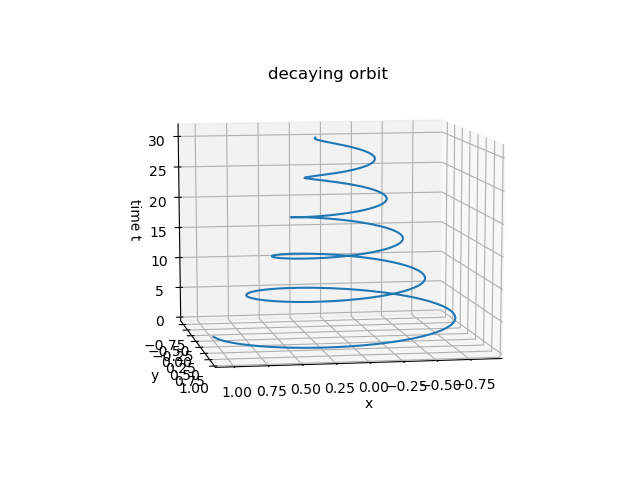
\includegraphics[width=.7\linewidth]{./gfx/plt-orbit3D}
	\captionof{figure}{3D-Kurve}
\end{center}
\end{tcolorbox}


\subsection{Plots von Flächen}
Für die Darstellung von Flächen im Dreidimensionalen muss die Zuordnung von X-Y-Koordinaten zur Z-Koordinate derselben Logik folgen wie bei den Vektorfeldern (siehe Seite \pageref{ssc:vecFields}): Wir brauchen zwei \emph{zweidimensionale Arrays} \texttt{X, Y}, die so das \emph{Meshgrid} aufspannen. \texttt{X[i][j]} enthält dann die X-Koordinate des \texttt{i}-ten Punkts in Zeilenrichtung und des \texttt{j}-ten Punkts in Spaltenrichtung. Gleiches gilt für \texttt{Y} bezüglich der Y-Koordinaten.

Die zugeordneten Daten \texttt{Z} müssen als \emph{zweidimensionales NumPy-Array} vorliegen. Im Detail wird das Modul \texttt{numpy} erst in Kapitel \ref{chp:Numpy} besprochen; es kann jedoch direkt aus einer \emph{zweidimensionalen} \inPy{list} über den Konstruktor von \texttt{numpy.array} erzeugt werden.

Der folgende Code erzeugt die Daten, die wir in den weiteren Beispielen für die Plots verwenden werden:
\begin{codebox}[Beispiel: Datenerzeugung: Sattelfläche]
\begin{minted}[linenos]{python3}
import numpy as np

W = 20
H = 30

func = lambda x, y : x**2 - y**2

X = [[j/10 - 1.0 for j in range(W)] for i in range(H)]
Y = [[i/10 - 1.5 for j in range(W)] for i in range(H)]
Z = [[None for i in range(W)] for j in range(H)]

for   i in range(H) :
  for j in range(W) :
    x = X[i][j]
    y = Y[i][j]
    Z[i][j] = func(x, y)

Z=np.array(Z)
\end{minted}
\end{codebox}

\begin{tcolorbox}[title=Sneak Preview: NumPy]
Die Plot-Daten können mit dem Modul \texttt{numpy} auch so erzeugt werden:

\vspace{6pt}
\begin{codebox}[Beispiel: Datenerzeugung: Sattelfläche mit \texttt{numpy}]
\begin{minted}[linenos]{python3}
import numpy as np

X, Y = np.meshgrid(np.linspace(-1, 1, 20), np.linspace(-1.5, 1.5, 30))
Z = X**2 - Y**2
\end{minted}
\end{codebox}

In Kapitel \ref{chp:Numpy} wird dies im Detail besprochen.
\end{tcolorbox}

\subsubsection{Wireframes}
Wireframes oder Drahtgittermodelle zeichnen Datenpunkte jeweils verbunden mit ihren nächsten Nachbarn. Die Flächen zwischen diesen Verbindungslinien bleiben transparent. Der Befehl zum Erstellen eines Drahtgittermodells ist \texttt{plot\_wireframe(X, Y, Z)}:

\begin{codebox}[Beispiel: Drahtgittermodell, width=.55\linewidth, nobeforeafter, equal height group = grpXmpWireframe]
\begin{minted}[linenos]{python3}
import matplotlib.pyplot as plt
from mpl_toolkits.mplot3d import Axes3D

fig = plt.figure()
drw = fig.add_subplot(
    111,
    projection='3d'
)

drw.plot_wireframe(X, Y, Z)

plt.show()
\end{minted}
\end{codebox}
%
\begin{tcolorbox}[title=Ausgabe: Drahtgittermodell, width=.45\linewidth, nobeforeafter, equal height group = grpXmpWireframe]
	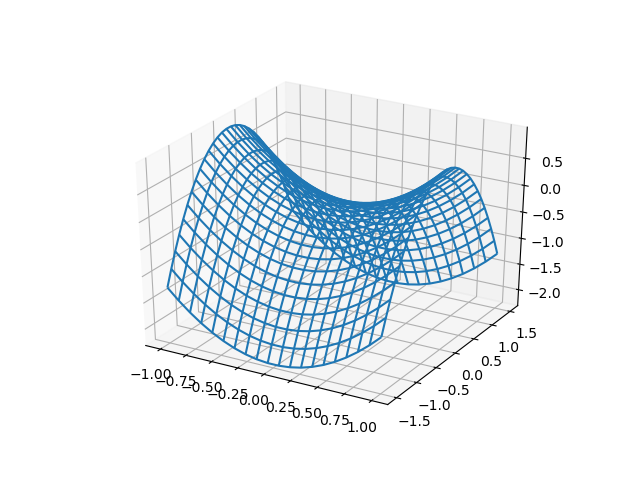
\includegraphics[width=\linewidth]{./gfx/plt-wireframe}
	\captionof{figure}{Drahtgittermodell}
\end{tcolorbox}
Siehe auch \url{https://matplotlib.org/3.1.1/api/_as_gen/mpl_toolkits.mplot3d.axes3d.Axes3D.html?highlight=plot_wireframe} für weitere Details.

\subsubsection{Surface Plots}
Surface Plots oder ausgefüllte Drahtgittermodelle erreichen sie, indem Sie den Befehl \texttt{plot\_wireframe} durch \texttt{plot\_surface} ersetzen. Er folgt denselben Regeln wie \texttt{plot\_wireframe}, unterstütz jedoch andere optionale Parameter, die Sie unter \url{https://matplotlib.org/api/_as_gen/mpl_toolkits.mplot3d.axes3d.Axes3D.html?highlight=plot_surface} nachschlagen können. Unterstützt werden auch Schattierungs und Transparenz-Effekte.

\begin{codebox}[Beispiel: Ausgefülltes Drahtgittermodell, width=.55\linewidth, nobeforeafter, equal height group = grpXmpSurface3D]
\begin{minted}[linenos]{python3}
import matplotlib.pyplot as plt
from mpl_toolkits.mplot3d import Axes3D

fig = plt.figure()
drw = fig.add_subplot(
    111,
    projection='3d'
)

drw.plot_surface(X, Y, Z)

plt.show()
\end{minted}
\end{codebox}
%
\begin{tcolorbox}[title=Ausgabe: Ausgef. Drahtgittermodell, width=.45\linewidth, nobeforeafter, equal height group = grpXmpSurface3D]
	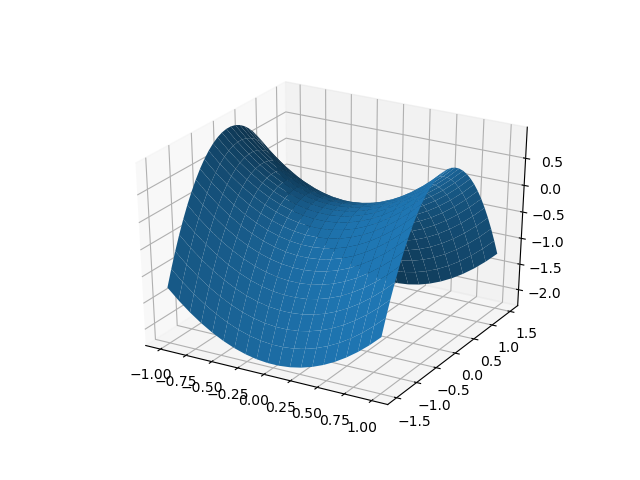
\includegraphics[width=\linewidth]{./gfx/plt-surface3D}
	\captionof{figure}{Ausgefülltes Drahtgittermodell}
\end{tcolorbox}

\subsubsection{Flache 3D-Darstellung mit Falschfarben und als Kontourplot}
Wie schon angesprochen können 3D-Darstellungen oft schwerer zu lesen sein. Teile des Plots sind \enquote{hinter} anderen verborgen, und auf den schräg über die Zeichenebene verlaufenden Achsen sind Werte oft schwerer exakt abzulesen. Eine beliebte Alternative sind daher Falschfarben-Darstellungen und Konturlinien.

Mit der Methode \texttt{pcolor} lässt sich eine einrache Falschfarbendarstellung dreidimensionaler Daten erreichen. Wie schon bei \texttt{plot\_wireframe} und \texttt{plot\_surface} müssen nur die X-, Y- und Z-Daten übergeben werden. Jeder Punkt in der X-Y-Ebene wird durch ein Rechteck in einer bestimmten Farbe dargestellt. Die Farbe richtet sich dabei nach dem Z-Wert. Der Rückgabewert von \texttt{pcolor} ist ein \texttt{matplotlib.collections.PolyCollection}-Objekt und kann \ua dazu genutzt werden, um eine Farblegende zu erstellen. Hierzu dient die Methode \texttt{colorbar}. Sie wirkt auf ein \texttt{Figure}-Objekt, und fügt eine Farblegende zum zuletzt auf dieser \texttt{Figure} gezeichneten Sublot eine Farbskala hinzu. Als Parameter wird dabei ein Objekt erwartet, aus dem diese Farbskala erzeugt werden kann -- beispielsweise eben der Rückgabewert von \texttt{pcolor}.

Die Methode \texttt{contour} zeichnet aus den X- Y- und Z-Daten eine Karte von \enquote{Höhenlinien}, \ie Linien, entlang derer der Z-Wert konstant bleibt. \enquote{Zwischen} den Gitterpunkten wird interpoliert.

Die Methode \texttt{contourf} schließlich erzeugt ebenfalls Höhenlinien, füllt aber die Flächen zwischen diesen Linien farbig aus. Lesen Sie diesen Befehl also am besten als \emph{contour-filled}. Auf diese Art lässt sich eine \enquote{glattere} Darstellung als mit \texttt{pcolor} erreichen. Natürlich ist dies nicht immer auch so erwünscht.

Weitere Details zu den Methoden finden Sie unter
\begin{itemize}
\item \url{https://matplotlib.org/3.1.1/api/_as_gen/matplotlib.axes.Axes.pcolor.html}
\item \url{https://matplotlib.org/3.1.1/api/_as_gen/matplotlib.pyplot.contour.html}
\item \url{https://matplotlib.org/3.1.1/api/_as_gen/matplotlib.pyplot.contourf.html}
\end{itemize}

\begin{codebox}[Beispiel: Darstellung in Falschfarben und als Kontourplot]
\begin{minted}[linenos]{python3}
import matplotlib.pyplot as plt

fig = plt.figure(figsize=(12,4))
grd = fig.add_gridspec(1, 7)

drw = fig.add_subplot(grd[0,0:2])
drw.set_title("pcolor")
col = drw.pcolor(X, Y, Z)

drw = fig.add_subplot(grd[0,2:4])
drw.set_title("contour")
drw.set_yticks([])
drw.contour(X, Y, Z)

drw = fig.add_subplot(grd[0,4:6])
drw.set_title("contourf")
drw.set_yticks([])
drw.contourf(X, Y, Z)

drw = fig.add_subplot(grd[0,6])
drw.axis("off")
fig.colorbar(col)

plt.show()
\end{minted}
\end{codebox}
%
\begin{tcolorbox}[title=Ausgabe: Darstellung in Falschfarben und als Kontourplot]
	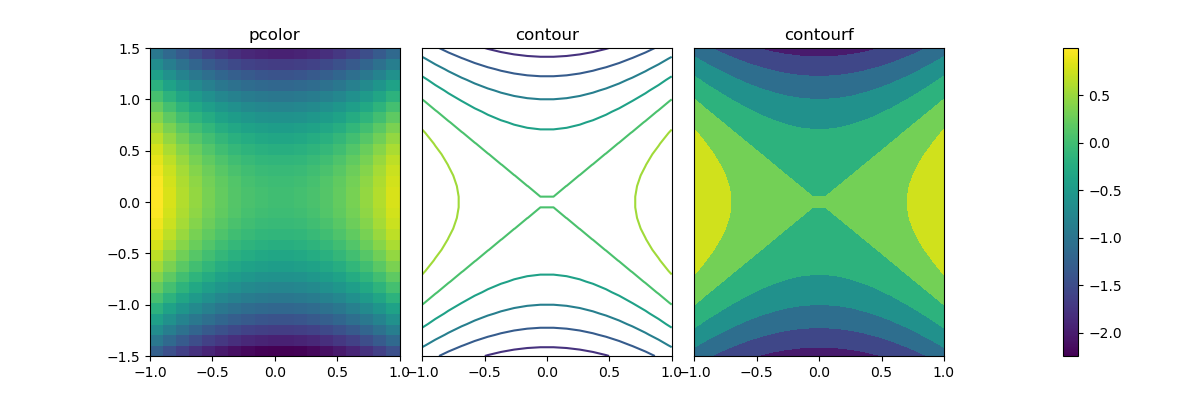
\includegraphics[width=\linewidth]{./gfx/plt-falseColour}
	\captionof{figure}{Darstellung in Falschfarben und als Kontourplot}
\end{tcolorbox}

\section{Ausgabe in Dateien}
Die Graphen, die Sie mit der MatPlotLib erzeugen, können Sie auch direkt als Grafik-Dateien abspeichern. Hierzu dient der Befehl \texttt{plt.savefig} bzw. die Methode \texttt{savefig}.

Der Methode \emph{muss} ein Dateiname als erster Parameter übergeben werden. Eine Datei mit entsprechendem Namen wird angelegt, falls sie noch nicht existiert; sollte eine Datei mit dem angegebenen Namen bereits existieren, wird diese ohne weitere Nachfrage überschrieben.

Optional kann auch mit dem Parameter \texttt{format} ein String übergeben werden, der das Dateiformat festlegt. Unterstützt werden die Formate eps, pdf, pgf, png, ps, raw, rgba, svg und svgz. Der Default-Wert ist \inPy{"png"}; jedoch versucht die MatPlotLib aber auch, aus dem Dateinamen ein geeignetes Format abzuleiten. Wird kein Format explizit angegeben, wird die Erweiterung des Dateinamens zur Bestimmung des Dateityps herangezogen. Beispielsweise führt \texttt{fig.savefig("filename.pdf")} eine PDF mit dem Namen \texttt{filename.pdf} erzeugen. Dagegen liefert \texttt{fig.savefig("filename.pdf", format="png")} dazu, dass eine PNG mit dem Dateinamen \texttt{filename.pdf} geschrieben wird.

Sehen Sie sich auch die Dokumentation unter \url{https://matplotlib.org/3.1.1/api/_as_gen/matplotlib.figure.Figure.html?highlight=savefig#matplotlib.figure.Figure.savefig} an für weitere Details.

\begin{hintbox}[Speicherbedarf]
In Python ist es sehr leicht, große Datenmengen zu generieren, und damit sogar zeitweise seinen Rechner komplett auszulasten. Dies sollte insbesondere bedacht werden, wenn mit Plots gearbeitet wird.

Die MatPlotLib speichert intern keine Bilder, sondern wirklich die Rohdaten. Das bedeutet, dass zu jedem Punkt einer Kurve sowohl X- als auch Y-Koordinate gespeichert werden müssen. Da diese Informationen \idR als \inPy{float} vorliegen, sind dies also mindestens 16 Byte pro Datenpunkt. Ggf. kommen zusätzliche Daten für Formatierungen etc. hinzu. Eine Kurve mit \SI{1000000}{} Datenpunkten (nicht ungewöhnlich für wissenschaftliche Simulationen) belegt also bereits \SI{16}{MB} im Arbeitsspeicher, auch wenn das daraus errechnete Bild nur wenige \SI{100}{kB} belegt.
\end{hintbox}
%
\begin{hintbox}[]
Weiter liegen die Daten oft doppelt im Arbeitsspeicher vor. Betrachten Sie folgenden Code-Auszug:

\begin{codebox}[Beispiel: Daten-Dopplung]
\begin{minted}[]{python3}
import matplotlib.pyplot as plt

X = [x * .001 for x in range(1000000)]
Y = [0]
for x in X[1:] :
    Y.append( (Y[-1] ** 2 - .0005 * x) % 2 )

plt.plot(X, Y, ",")
plt.show()
\end{minted}
\end{codebox}
Die \inPy{list}s \texttt{X, Y} werden durch den Befehl \texttt{plot} tatsächlich in einen von der MatPlotLib verwalteten Speicherbereich \emph{kopiert}! Kurzfristig verbrauchen wir hier also \SI{32}{MB} an Arbeitsspeicher für eine einzige Kurve.

Wenn wir verschiedene Parameter in unserer Simulation durchtesten, kann der Speicherbedarf schnell anwachsen. Anforderungen im Gigabyte-Bereich sind leicht erreicht.

Um dieses Problem zu umgehen, können wir versuchen, unsere Simulation so aufzubauen, dass sie Daten nicht am Stück generiert, sondern jeweils in kleineren Batches. Aus diesen Batches wird nur eine Untermenge ausgewählt, die tatsächlich geplottet wird; der Rest dagegen wird wieder verworfen:

\begin{codebox}[Beispiel: Batch-Weise Berechnung und reduziertes Plotten]
\begin{minted}[]{python3}
import matplotlib.pyplot as plt

Y = [0]
for batch in range(1000) :
    X = [x * .001 for x in range(batch * 1000, (batch + 1) * 1000)]
    for x in X[1:] :
        Y.append( (Y[-1] ** 2 - .0005 * x) % 2 )
    
    plt.plot(X[::50], Y[::50], "b,")
    
    Y = [(Y[-1] ** 2 - .0005 * x) % 2]
plt.show()
\end{minted}
\end{codebox}

Im zweiten Beispiel sinkt der Speicherbedarf vom \SI{32}{MB} auf nur knapp über \SI{46}{kB}. Manchmal bringt ein solches Reduzieren der zu plottenden Datenmenge zusätzlich den Vorteil, dass die innere Struktur der Plots leichter erkennbar wird, wie die Gegenüberstellung der beiden Ausgaben zeigt:
\end{hintbox}
%
\begin{hintbox}[]
\begin{center}
	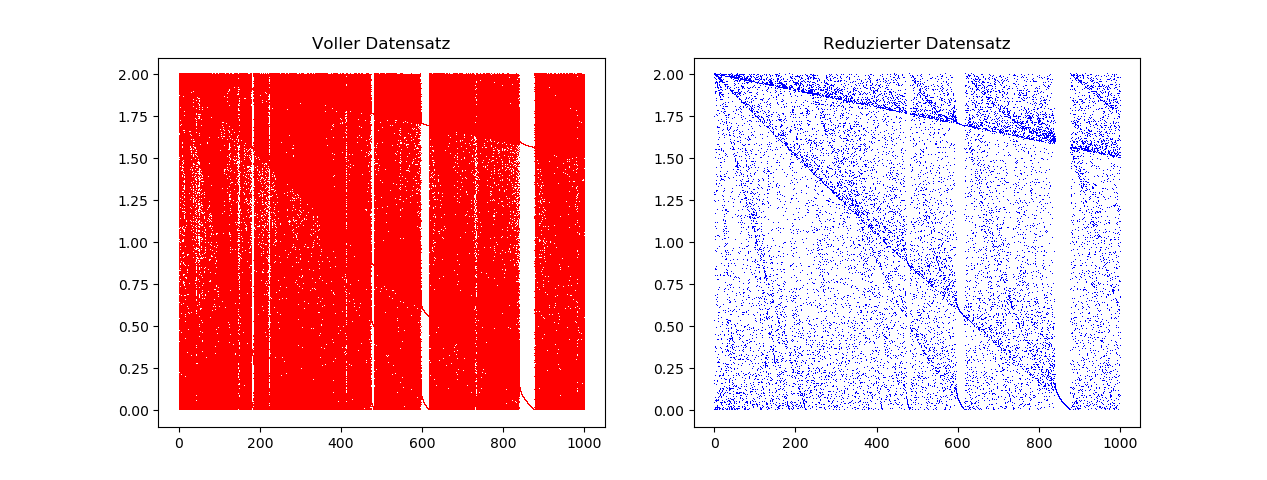
\includegraphics[width=.9\linewidth]{./gfx/plt-chaos-reduced}
	\captionof{figure}{Deterministisches Chaos: Voller Datensatz und Reduzierter Datensatz}
\end{center}

Das Beispiel ist lose angelehnt an die Erkenntnisse, die ich aus dem Kurs \emph{Chaos and Nonlinear Dynamics} an der Universität Regensburg gewonnen habe.
\end{hintbox}
